%http://www.maths.manchester.ac.uk/~kd/latextut/pdfbyex.htm
\documentclass[a4paper,twoside]{book}      % Comments after  % are ignored
\usepackage{amsmath,amssymb,amsfonts} % Typical maths resource packages
\usepackage{graphics}                 % Packages to allow inclusion of graphics
\usepackage{graphicx}
\usepackage{color}                    % For creating coloured text and background
\usepackage{hyperref}                 % For creating hyperlinks in cross references
\usepackage{listings}
\usepackage{tabularx}

\usepackage{color}
\usepackage{listings}
%\usepackage{textcomp}
\usepackage{setspace}
%\usepackage{palatino}

\newenvironment{codelisting0}
{\begin{list}{}{\setlength{\leftmargin}{1em}}\item\tiny}
{\end{list}}

\renewcommand{\lstlistlistingname}{Code Listings}
\renewcommand{\lstlistingname}{Code Listing}
\definecolor{orange}{rgb}{1,0.5,0}
\definecolor{gray}{gray}{0.5}
\definecolor{green}{rgb}{0,0.5,0}
\definecolor{lightgreen}{rgb}{0,0.7,0}
\definecolor{purple}{rgb}{0.5,0,0.5}
\definecolor{darkred}{rgb}{0.5,0,0}

%%% ----- commented out -------- Philipp --- 2010-11-09 ----------
%%%\lstnewenvironment{code}[1][]{
%%%\lstset{ %
%%%language=XML,                % choose the language of the code
%%%basicstyle=\footnotesize,       % the size of the fonts that are used for the code
%%%numbers=left,                   % where to put the line-numbers
%%%numberstyle=\footnotesize,      % the size of the fonts that are used for the line-numbers
%%%stepnumber=1,                   % the step between two line-numbers. If it's 1 each line will be numbered
%%%numbersep=5pt,                  % how far the line-numbers are from the code
%%%backgroundcolor=\color{black},  % choose the background color. You must add \usepackage{color}
%%%showspaces=false,               % show spaces adding particular underscores
%%%showstringspaces=false,         % underline spaces within strings
%%%showtabs=false,                 % show tabs within strings adding particular underscores
%%%frame=single,                   % adds a frame around the code
%%%tabsize=2,                      % sets default tabsize to 2 spaces
%%%captionpos=b,                   % sets the caption-position to bottom
%%%breaklines=true,                % sets automatic line breaking
%%%breakatwhitespace=false,        % sets if automatic breaks should only happen at whitespace
%%%caption = OWL encoding of a small persons and movie genres ontology.,
%%%label=lst:owlExample
%%%}}{}

\newenvironment{codelisting}
{\begin{list}{}{\setlength{\leftmargin}{1em}}\item}
{\end{list}}

\definecolor{darkgray}{rgb}{0.95,0.95,0.95}
\lstset{language=Java}
%\lstset{basicstyle=22}
\lstset{backgroundcolor=\color{darkgray}}
\lstset{numbers=left, numberstyle=\tiny, stepnumber=1, numbersep=5pt}
\lstset{keywordstyle=\color{red}}
\lstset{showspaces=false}
\lstset{commentstyle=\color{green}}
\lstset{stringstyle=\color{blue}}
\lstset{basicstyle=\small\tt}
\lstset{numberstyle=\scriptsize\tt}
\lstset{showstringspaces=false}
\lstset{captionpos=b}

\newenvironment{mytinylisting}
{\begin{list}{}{\setlength{\leftmargin}{1em}}\item\tiny\bfseries}
{\end{list}}




\oddsidemargin 0cm
\evensidemargin 0cm

\pagestyle{myheadings}         % Option to put page headers
                               % Needed \documentclass[a4paper,twoside]{article}
\markboth{{\small\it Overview of TUD Palladian}}
{{\small\it David Urbansky, Klemens Muthmann, Philipp Katz} }

%A4 settings
\textwidth 15.5cm
\textheight 24cm

%A5 settings
%\textwidth 10.0cm
%\textheight 17cm
\topmargin -1cm
\parindent 0cm

\parskip 1mm
\newtheorem{theorem}{Theorem}[section]
\newtheorem{proposition}[theorem]{Proposition}
\newtheorem{corollary}[theorem]{Corollary}
\newtheorem{lemma}[theorem]{Lemma}
\newtheorem{remark}[theorem]{Remark}
\newtheorem{definition}[theorem]{Definition}

\def\R{\mathbb{ R}}
\def\S{\mathbb{ S}}

\date{\today}
%\title{\fcolorbox{red}{blue}{\color{white}Including colour, pdf graphics and hyperlinks
%\footnote{A demonstration example including colored text and graphics}}}
\title{TUD Palladian Overview}
\author{David Urbansky, Klemens Muthmann, Philipp Katz \\
{\small TU Dresden, Department of Systems Engineering, Chair Computer Networks, IIR Group, Germany}
}
%\author{David Urbansky \\
%{\small TU Dresden, Department of Systems Engineering, Chair Computer Networks, IIR Group, Germany}
%}
%\author{Klemens Muthmann \\
%{\small TU Dresden, Department of Systems Engineering, Chair Computer Networks, IIR Group, Germany}
%}
\usepackage{fix-cm}
\usepackage[absolute]{textpos}
\newcommand{\bigsize}{\fontsize{18pt}{10pt}\selectfont}
\newcommand{\titleelementsize}{\fontsize{12pt}{10pt}\selectfont}
\begin{document}
%\maketitle
%\begin{abstract}
%This document explains basic functionalities of the TUDIIR Toolkit. Its intention is to explain (new) developers how to work with the toolkit and how to extend its capabilities.
%\end{abstract}

\begin{titlepage}
\centering


{\bigsize TUD Palladian Overview} \\

\vspace{1.5cm}

{\titleelementsize David Urbansky, Klemens Muthmann, Philipp Katz} \\
\vspace{0.1cm}
{\small TU Dresden, Department of Systems Engineering, Chair Computer Networks, IIR Group, Germany} \\
\vspace{0.8cm}
{\titleelementsize \today} \\
\vspace{2cm}

\includegraphics[width=0.5\textwidth]{img/logo.png}

\end{titlepage}



\tableofcontents

\chapter{Introduction}
Internet Information Retrieval (IIR) is a research domain in computer science concerned with the retrieval, extraction, classification, and presentation of information from the Internet. The toolkit provides functionality which is often needed to perform IIR tasks such as crawling, classification, and extraction of various types of information.

\section{What Palladian is}
%TODO contributions
Palladian is a collection of algorithms for text processing focused on \textbf{ classification}, \textbf{ extraction}, and \textbf{ retrieval}. The concept of Palladian is system to reuse algorithms that are freely available and build upon them to drive research. When trying to learn and advance in a new field of research, one has to play around with many code snippets from various authors, this toolkit tries to ease this process by making external libraries accessible through a single interface. This way new algorithms can be quickly compared to the state-of-the-art.
The best results from students at the Dresden University of Technology find their way into the toolkit allowing other users to create more advanced programs in the future.

Our main contributions to the research community are:
\begin{enumerate}
\item New algorithms in the fields of classification and extraction that can easily be tested and applied to other projects.
\item Single interface access to bundles of well established algorithms.
\item Helping make research more transparent by fomenting users to reproduce results with the included algorithms.
\end{enumerate}

Figure \ref{fig:architecture} shows the main packages of Palladian. The focus is evidently on retrieval (Crawler, API access, feed reading...), preprocessing (tokenization, sentence splitting...), classification (KNN, Dictionary Classifier...), and extraction (named entities, tags...).

\begin{figure}[ht!]
\centering
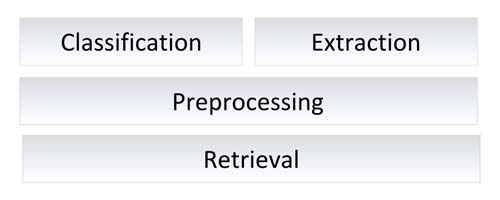
\includegraphics[width=0.6\textwidth]{img/architecture.pdf}
\caption{Important Packages of Palladian.}
\label{fig:architecture}
\end{figure}

\section{What Palladian is NOT}
Palladian is not a full natural language processing suite nor does it contain a \textit{ full} set of algorithms in the fields of classification, extraction, and information retrieval. Palladian is not a commercial product either, we like to answer questions as soon and comprehensive as possible but cannot guarantee this support.

\section{Who the Intended User is}
In general everybody is welcome to use Palladian, but the researchers that would develop algorithms and would like to quickly test or compare them are the focus. Researchers likely to help other researchers, that won't mind a software that is not perfect, bug-free or commercial.

\section{License}
The complete source code is licensed under the Apache License 2.0. All source files should include the following license snippet at the very top.

\begin{verbatim}
Copyright 2010 David Urbansky, Klemens Muthmann
Licensed under the Apache License, Version 2.0 (the "License"); you may not
use this file except in compliance with the License. You may obtain a copy of
the License at

http://www.apache.org/licenses/LICENSE-2.0

Unless required by applicable law or agreed to in writing, software
distributed under the License is distributed on an "AS IS" BASIS, WITHOUT
WARRANTIES OR CONDITIONS OF ANY KIND, either express or implied.
See the License for the specific language governing permissions and
limitations under the License.
\end{verbatim}

\section{Evaluation Measures for IIR Systems}

This sections outlines important evaluation measures which are typically used for comparing and scoring algorithms and techniques in (Internet) Information Retrieval. Our goal is to give just a brief overview, more details can be found in the referenced literature.

% TODO ... work for the holidays

\subsection{Precision, Recall, F-Measure}

\begin{figure}[ht!]
\centering
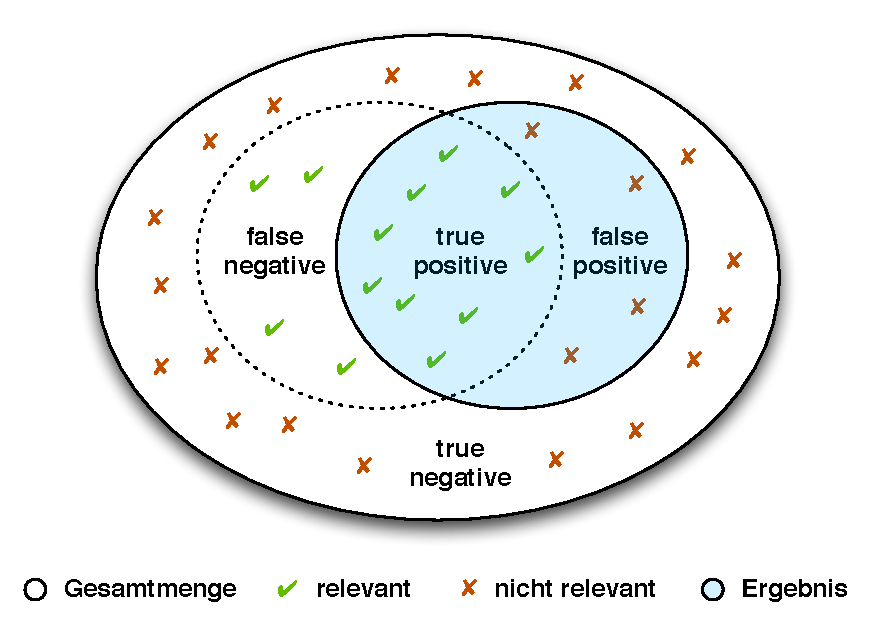
\includegraphics[width=0.6\textwidth]{img/PrecisionRecallMengen.pdf}
\caption{Set of Documents as Basis for Precision and Recall.}
\label{fig:PrecisionRecall}
\end{figure}

\subsection{Mean Squared Error, Root Mean Squared Error}

\subsection{Mean Average Precision}

\subsection{Mean Reciprocal Rank}

\section{Alternative and Complimentary Toolkits}
\label{sec:alternativesToPalladian}
Some functionalities of this toolkit are covered in other libraries. If you can't find the functionality you need in Palladian you might want to take a look at these alternatives. Some of the objectives of Palladian are to create new functionalities or improve existing ones, not to reinvent the wheel and redo work that functions well in other libraries.

%TODO clean up list, bullets or table of services
\begin{enumerate}
\item \textbf{AlchemyAPI} \cite{alchemyapi} is a commercial web-service that can be used via several programming languages. The service offers named entity recognition, text classification, language identification, concept tagging, keyword extraction, content scraping, and web page cleaning.
The service comes in 4 variants: free, basic, professional, and metered.
\item \textbf{Apache Mahout} \cite{settings2apache} is a Java-based machine learning library. Its main features are collaborative filtering, user and item based recommenders, (fuzzy k-means clustering, mean shift clustering, latent dirichlet process allocation, singular value decomposition, parallel frequent pattern mining, complementary naive bayes classifier, and a random forest decision tree based classifier.
The library is licensed under the Apache Software license.
\item \textbf{Balie} \cite{balie} is a Java-based information extraction library. Its main features are language identification, tokenization, sentence boundary detection, and named entity recognition (using dictionaries).
The library is licensed under the GNU GPL and supports English, German, French, Romanian, and Spanish as input languages.
\item \textbf{ContentAnalyst} \cite{contentanalyst} is a commercial platform for text analytics. The platform's main features are concept search, dynamic clustering, near-duplicate document identification, automatic summarization, text classification, and latent semantic indexing.
\item The \textbf{Dragon Toolkit} \cite{zhou2007dragon} is a Java-based development package for information retrieval and text mining. Its main features are text classification, text clustering, text summarization, and topic modeling.
\item \textbf{FreeLing} \cite{atserias2006freeling} is a natural language processing library written in C++. Its main features are Text tokenization, sentence splitting, morphological analysis, sSuffix treatment, retokenization of clitic pronouns, flexible multiword recognition, contraction splitting, probabilistic prediction of unkown word categories, named entity detection, recognition of dates, numbers, ratios, currency, and physical magnitudes, PoS tagging, chart-based shallow parsing, named entity classification,  WordNet based sense annotation and disambiguation, Rule-based dependency parsing, and nominal correference resolution.
It is licensed under GPL and supports Spanish, Catalan, Galician, Italian, English, Welsh, Portuguese, and Asturian as languages. An online demo is available under \url{http://garraf.epsevg.upc.es/freeling/demo.php}.
\item \textbf{GATE} \cite{cunningham2002gate} is a Java-based text mining and processing framework. The framework itself comes with few text processing features but many plugins can be used and chained into a text engineering pipeline.
The framework is licensed under the GNU Lesser General Public License.
\item The \textbf{Illinois Cognitive Computation Group} \cite{illinoisccg} has a list of ready to use programs for semantic role labeling, text chunking, named entity tagging, named entity discovery, PoS tagging, unsupervised rank aggregation, and named entity similarity metrics.
\item \textbf{Julie NLP} \cite{tomanek2007uima,hahn2008overview} is a Java-based toolkit of UIMA based text processing components. The toolkit can be used for semantic search, information extraction, named entity recognition, and text mining.
The Toolkit is licensed under the Common Public License.
\item \textbf{Language Computer} \cite{lanuagecomputer} provides commercial products for sentence splitting, tokenization, PoS tagging, named entity recognition, co-reference resolution, attribute extraction, relationship extraction, event extraction, question answering, and text summarization.
\item \textbf{Lemur Project} \cite{lemur} provides a toolkit with search engines and tools for research tasks in information retrieval and text mining. The project was founded in 2000 by the Center for Intelligent Information Retrieval (CIIR) at the University of Massachusetts, Amherst. Updates for the toolkit are released on a regular basis. The toolkit is written in C++, but also offers C\# and Java APIs. Beside the Lemur toolkit itself, the project offers a search engine called ``Indri'' and a browser plugin to capture users' query and browsing behaviours.
\item \textbf{Lingo3G} \cite{lingo3g} is a text clustering engine that organizes text collections into hierarchical clusters.
The software is commercial but \cite{stefanowski2003carrot} offers an open source alternative for text clustering algorithms written in Java. The algorithms integrate with other programming or scripting languages such as PHP, Ruby, and C\# too.
\item \textbf{LingPipe} \cite{lingpipe} is a text processing toolkit using computational linguistics. LingPipe is written in Java. Its main features are topic classification, named entity recognition, clustering, PoS tagging, sentence detection, spelling correction, database text mining, string comparisons, interesting phrase detection, character language modeling, chinese word segmentation, hyphenation and syllabification, sentiment analysis, language identification, singular value decomposition, logistic regression, expectation maximization, and word sense disambiguation.
LingPipe is available under a free license for academic use and several commercial licenses.
\item \textbf{Mallet} \cite{mccallum2002mallet} is a Java-based toolkit for statistical natural language processing. Its main features are text classification, sequence tagging (PoS tagging), topic modeling, and numerical optimization.
The toolkit is licensed under the Common Public License.
\item \textbf{MinorThird} \cite{cohen2004minorthird} is a Java-based toolkit for text processing. Its main features are annotating text, named entity recognition, and text classification.
The toolkit is licensed under the BSD license.
\item \textbf{MontyLingua} \cite{liu2004montylingua} is a Python and Java-based toolkit for natural language processing (English only). Its main features are tokenization, PoS tagging, lemmatization, and natural language summarization.
The toolkit is free for non-commercial use and licensed under the MontyLingua version 2.0 License.
\item \textbf{MorphAdorner} \cite{morphadorner} is a Java-based command line program for text processing. Its main features are language recognition, lemmatization, name recognition, PoS tagging, noun pluralization, sentence splitting, spelling standardization, text segmentation, verb conjugation, and word tokenization.
The program is licensed under a NCSA style license.
\item \textbf{NaCTeM Software Tools} \cite{nactem} are programs for natural language processing and text mining that are made available by the National Centre for Text Mining. The programs include functionality for PoS tagging, syntactic parsing, named entity recognition, sentence splitting, text classification, and sentiment analysis.
\item \textbf{NLTK} \cite{loper2002nltk} is a Python-based natural language processing toolkit. Its main features are tokenization, stemming, PoS tagging, text classification, and syntactic parsing.
The toolkit is licensed under the Apache 2.0 license.
\item \textbf{OpenCalais} \cite{opencalais} is a web service that performs named entity recognition, fact and event extraction.
The web service is free for commercial and non-commercial use but limited to 50,000 transactions a day. A professional plan is available too including more transactions and an service license agreement.
\item \textbf{OpenNLP} \cite{opennlp} is a toolkit of various open source natural language processing packages. The goal of this toolkit is to integrate several stand-alone projects to increase the interoperability. Algorithms in this toolkit include but are not limited to tokenization and named entity recognition.
\item The \textbf{RASP System} \cite{briscoe2006second} is a C and Lisp-based toolkit for natural language processing (English only). Its main features are tokenization, PoS tagging, lemmatization, morphological analysis, and grammar-based parsing.
The toolkit is free for non-commercial use and licensed under the RASP System License.
\item The \textbf{Rosette Linguistic Platform} \cite{rosette} is a software suite that can perform name translation, name matching, named entity recognition, morphological analysis, and language identification. The suite works for 55 European, Asian, and Arabic languages.
The software is a commercial product.
\item \textbf{Stanford NLP} \cite{stanfordnlp} is a set of Java-based natural language processing libraries. Their main features are PoS tagging, named entity recognition, Chinese word segmentation, and classification.
The software distributions are licensed under the GNU Public License.
\item \textbf{SRILM -- The SRI Language Modeling Toolkit} \cite{stolcke2002srilm} is a C++-based toolkit for language modeling. Its main features are speech recognition, statistical tagging and segmentation, and machine translation.
The toolkit is free for non-commercial use and licensed under the SRILM Research Community License.
\item \textbf{TextAnalyst} \cite{textanalyst} is a commercial text processing software offering text summarization, semantic information retrieval, meaning extraction, and text clustering.
\item \textbf{VisualText} \cite{visualtext} is a natural language processing software that addresses named entity recognition, text indexing, text filtering, text classification, text grading, and text summarization.
\item \textbf{WEKA} \cite{hall2009weka} is a Java-based machine learning and data mining library. The library contains a large set of machine learning algorithms such as Support Vector Machines, Neural Networks, Naive Bayes, k-nearest neighbor for but not limited to (text) clustering, (text) classification, and regression.
The library is licensed under the GNU General Public License.
\end{enumerate}

\chapter{Installation and Making it Work}
Palladian depends on Java 1.6. If you are using Linux, make sure to use Sun's proprietary JDK instead of OpenJDK to avoid build problems\footnote{Open a Terminal and enter \texttt{java -version} to check the currently installed Java version. The necessary steps to change your Java version depend on your Linux distribution, for Ubuntu flavours see \url{https://help.ubuntu.com/community/Java}.}. The code base is managed using \href{http://subversion.apache.org/}{Subversion (SVN)} (see Chapter~\ref{sec:toolkitstructure}). It is build and tested automatically on every commit using \href{http://maven.apache.org/}{Apache Maven} and \href{http://hudson-ci.org/}{Hudson CI}. Bugs might be reported using the \href{http://www.redmine.org/}{Redmine bugtracker}. The project encoding is UTF-8. To support unavailable libraries we manage our own Maven repository using \href{http://nexus.sonatype.org/}{Sonatype Nexus}. How to use these components is explained in the next sections.

Currently each systems manages its own user base so registration is needed for each one. To start working with the toolkit you should send an E-Mail to a toolkit administrator to get access to the systems. Provide your name, the name of your advisor and the reason why you need to work with the toolkit and you will get your logins.
\section{Building Palladian using Apache Maven}
\label{sec:buildingthetoolkitusingapachemaven}
Apache \textbf{Maven needs to be installed} to build the toolkit. Instructions for how to \href{http://maven.apache.org/download.html#Installation}{install Maven} can be found in the link. There is one manual step before you can start building the toolkit. You need to add our Nexus repository to your local Maven settings. Do this by \textbf{locating or creating the settings.xml file in your local home folder:} \texttt{\%YOUR\_HOME\_FOLDER\%/.m2/settings.xml} and adding the following content, replacing both user and password as provided by the toolkit administrator:
\begin{verbatim}
<settings xmlns="http://maven.apache.org/SETTINGS/1.0.0"
  xmlns:xsi="http://www.w3.org/2001/XMLSchema-instance"
  xsi:schemaLocation="http://maven.apache.org/SETTINGS/1.0.0
                      http://maven.apache.org/xsd/settings-1.0.0.xsd">
  <servers>
    <server>
      <id>snapshots</id>
      <username>your-username</username>
      <password>your-password</password>
      <filePermissions>664</filePermissions>
      <directoryPermissions>775</directoryPermissions>
      <configuration></configuration>
    </server>
    <server>
      <id>releases</id>
      <username>your-username</username>
      <password>your-password</password>
      <filePermissions>664</filePermissions>
      <directoryPermissions>775</directoryPermissions>
      <configuration></configuration>
    </server>
  </servers>
</settings>
\end{verbatim}
You need to set your username and your password in the server section. This can be obtained by sending an E-Mail to \href{mailto:klemens.muthmann@tu-dresden.de}{klemens.muthmann@tu-dresden.de} stating who is your advisor and why you need to work with the toolkit. After completing the installation perform the following steps to build the toolkit using Maven:
\begin{enumerate}
\item Check out the code from SVN!
\item Open your favorite command line.
\item Change to the toolkits root folder.
\item Type \texttt{mvn clean install} to start the build process.
\end{enumerate}
There is also an \href{http://m2eclipse.sonatype.org/}{Eclipse plugin}, that allows you to issue maven build from within Eclipse. It is quite beta so it may present some issues.
\section{Regular Builds and Tests using Hudson CI}
Currently Palladian is build automatically every week using Hudson CI. Be careful to check in only working code or Hudson will send you and your advisor an E-Mail about broken code. If this happens try to fix your code as soon as possible and check it in again. You can get details about the problem by logging into \href{http://www.effingo.de/hudson}{Hudson}. You can get a login by sending an E-Mail stating your advisor and why you need to work with the toolkit to \href{mailto:klemens.muthmann@tu-dresden.de}{klemens.muthmann@tu-dresden.de}
\subsection{The Continuous Integration Game}
\label{sec:cigame}
Hudson supports a game that rewards people committing code that improves the toolkit and punishing people breaking it. The leader (the person having the most points) is highly valued by the toolkit committers community. The rules for the game are explained in detail in the next section.
\paragraph{Rules}
The rules of the game are:
\begin{itemize}
\item --10 points for breaking a build
\item 0 points for breaking a build that already was broken
\item +1 points for doing a build with no failures (unstable builds gives no points)
\item --1 points for each new test failures
\item +1 points for each new test that passes
\item Adding/removing a HIGH priority PMD warning = --5/+5. Adding/removing a MEDIUM priority PMD warning = --3/+3. Adding/removing a LOW priority PMD warning = --1/+1.
\item Adding/removing a violation = --1/+1. Adding/removing a duplication violation = +5/--5.
\item Adding/removing a HIGH priority findbugs warning = --5/+5. Adding/removing a MEDIUM priority findbugs warning = --3/+3. Adding/removing a LOW priority findbugs warning = --1/+1
\item Adding/removing a compiler warning = --1/+1.
\item Checkstyle Plugin. Adding/removing a checkstyle warning = --1/+1.
\end{itemize}

\section{Hello Toolkit -- Your First Application using Palladian}
\paragraph{Project creation:} Create a new Maven Project using the New Project wizard of Eclipse (See Fig.~\ref{fig:maven-project01},~\ref{fig:maven-project02} and \ref{fig:maven-project03}).
\begin{figure}
\centering
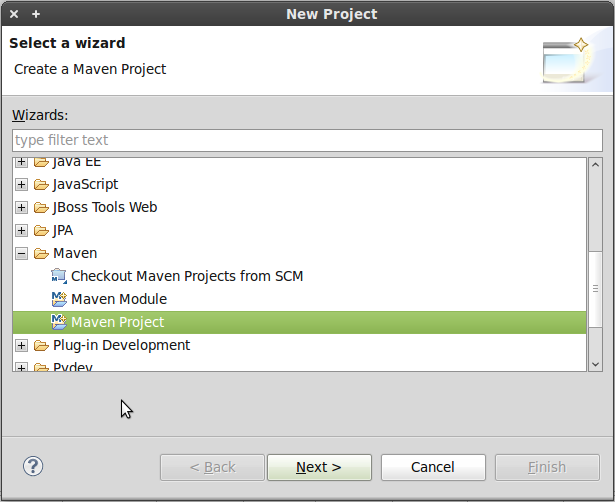
\includegraphics[width=\textwidth]{img/ht01.png}
\caption{Create a new Maven Project.}
\label{fig:maven-project01}
\end{figure}
\begin{figure}
\centering
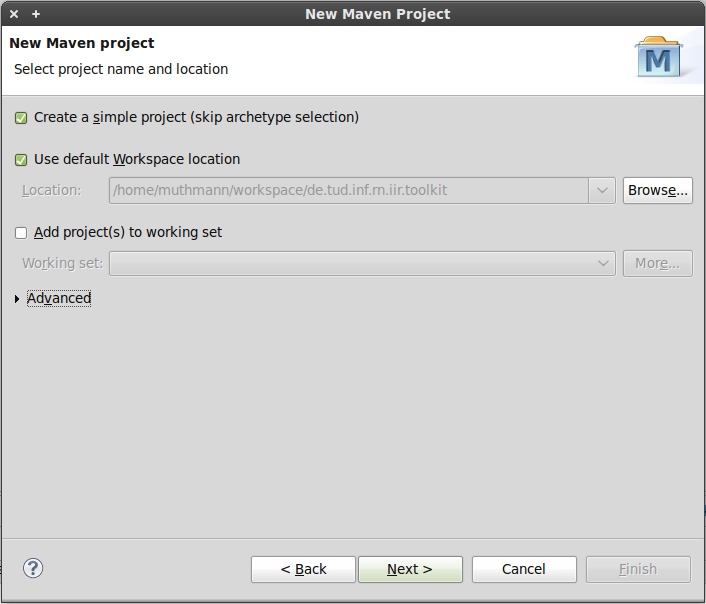
\includegraphics[width=\textwidth]{img/ht02.png}
\caption{Choose to create a simple Maven Project.}
\label{fig:maven-project02}
\end{figure}
\begin{figure}
\centering
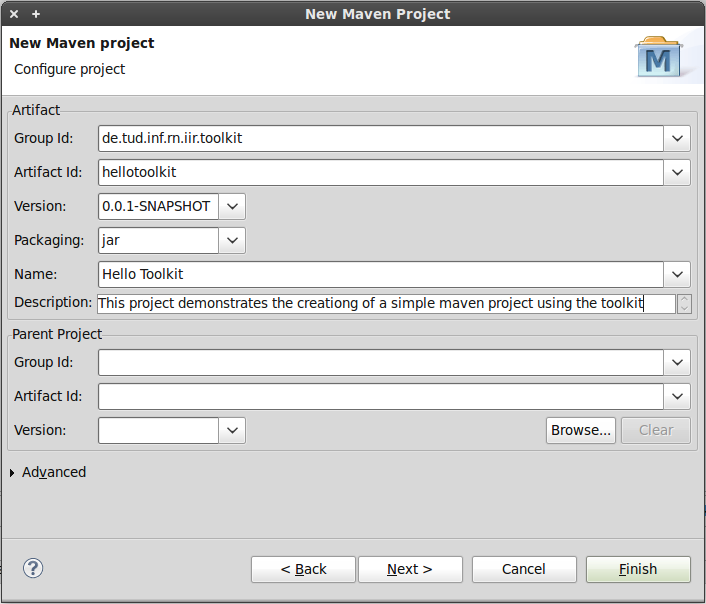
\includegraphics[width=\textwidth]{img/ht03.png}
\caption{Enter detail information about your new Maven Project}
\label{fig:maven-project03}
\end{figure}
\paragraph{Adding the toolkit dependency to the project:} Right click on the new project. In the context menu that appears choose \textit{Maven $\rightarrow$ Add Dependency} (See Fig.~\ref{fig:example-project-context-menu01} and \ref{fig:example-project-context-menu02}).
\begin{figure}
\centering
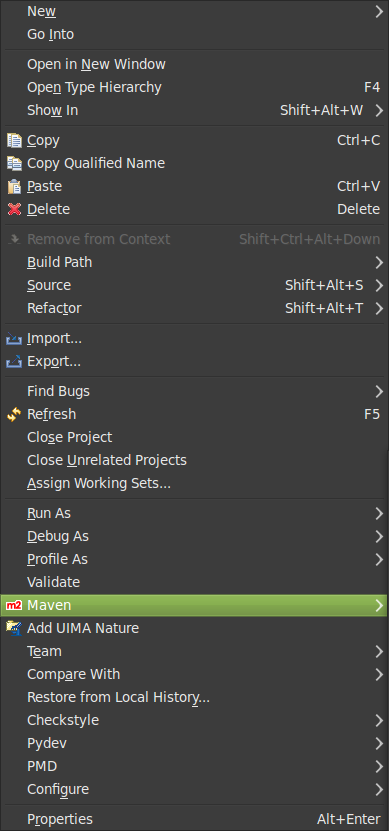
\includegraphics[scale=1]{img/context02.png}
\caption{Maven Project Context Menu. Choose \textit{Maven}}
\label{fig:example-project-context-menu01}
\end{figure}
\begin{figure}
\centering
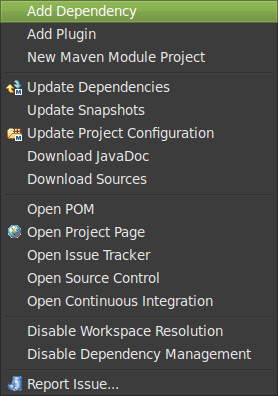
\includegraphics[scale=1]{img/context01.png}
\caption{Create a new Maven project}
\label{fig:example-project-context-menu02}
\end{figure}
A search interface appears (See~\ref{fig:add-dependency01}). If you followed the steps in Section~\ref{sec:buildingthetoolkitusingapachemaven} and installed the toolkit to your local Maven repository, you can type \textit{toolkit} in the search interface (See Fig.~\ref{fig:add-dependency02} and add the dependency with a double click on the \textit{de.tud.inf.rn.iir toolkit} entry. 

Note: If you need to add further dependencies in the future you can use the same steps.
\begin{figure}
\centering
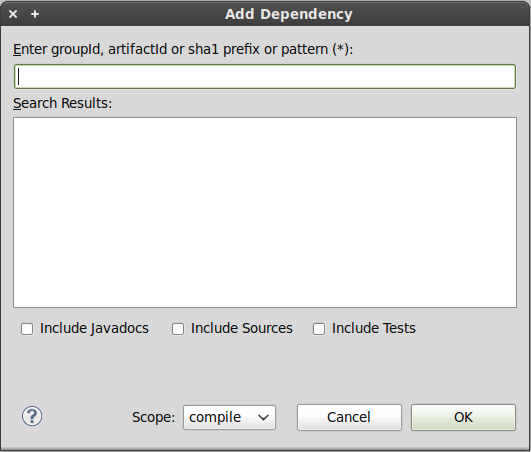
\includegraphics[width=\textwidth]{img/ht04.png}
\caption{Search interface for Maven dependencies.}
\label{fig:add-dependency01}
\end{figure}
\begin{figure}
\centering
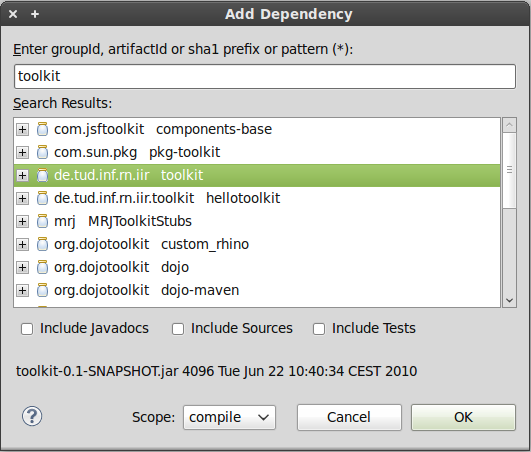
\includegraphics[width=\textwidth]{img/ht05.png}
\caption{Search results for \textit{toolkit}}
\label{fig:add-dependency02}
\end{figure}
The Maven plugin adds the dependency to your pom.xml file, which should look like Fig.~\ref{fig:pom01}.
\begin{figure}
\centering
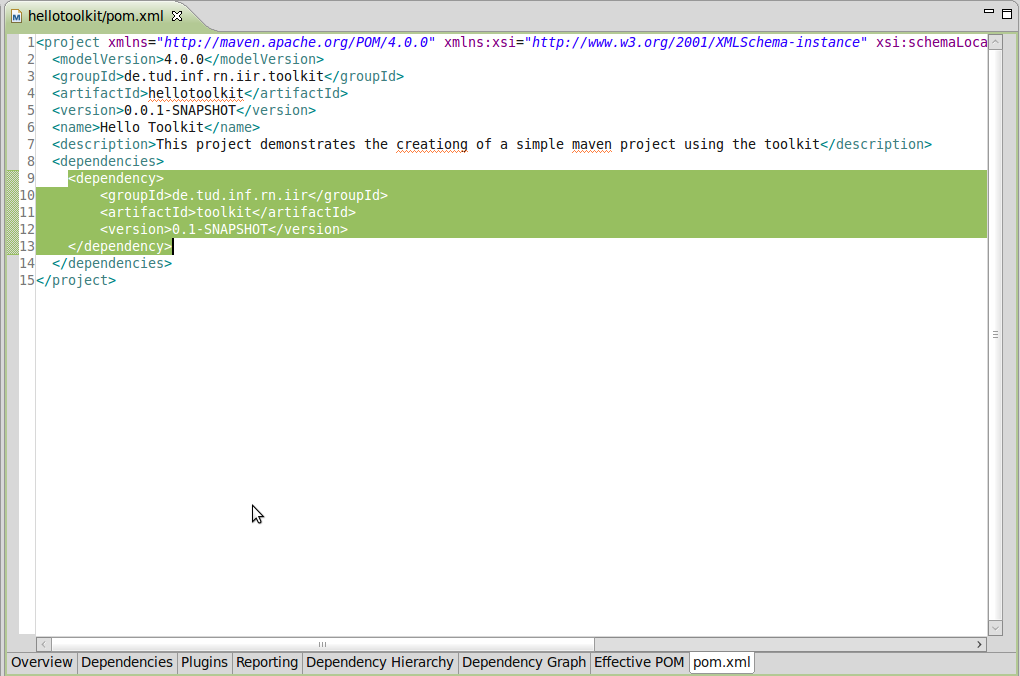
\includegraphics[width=\textwidth]{img/ht06.png}
\caption{POM with added dependency on the TUD Palladian toolkit.}
\label{fig:pom01}
\end{figure}
\paragraph{Configuring your project} Since Maven by default still uses Java 1.4 (conservative), but the toolkit depends on Java 1.6 (current) you need to configure the Maven Java compiler plugin to use Java 1.6 by adding the following markup to your pom.xml (add it after the description element):
\begin{verbatim}
<build>
 <plugins>
  <plugin>
   <groupId>org.apache.maven.plugins</groupId>
   <artifactId>maven-compiler-plugin</artifactId>
   <version>2.3.1</version>
   <configuration>
    <compilerArgument>-Xlint:all</compilerArgument>
    <showWarnings>true</showWarnings>
    <source>1.6</source>
    <target>1.6</target>
    <compilerArguments>
     <encoding>UTF-8</encoding>
    </compilerArguments>
    <showDeprecation>true</showDeprecation>
    <verbose>true</verbose>
    <encoding>UTF-8</encoding>
   </configuration>
  </plugin>
 </plugins>
</build>
\end{verbatim}
It is also necessary to tell Eclipse to use Java 1.6 instead of 1.4. To do this open the project properties via the context menu and choose \textit{Java Compiler} there change all three entries to 1.6. This is shown in Fig.~\ref{fig:java602} and Fig.~\ref{fig:java603}. The project's encoding needs to be set to UTF-8 which can be adjusted in the \textit{Resource} section as shown in Fig.~\ref{fig:utf8}. These properties can also be set for your whole workspace via Eclipse preferences.
\begin{figure}
\centering
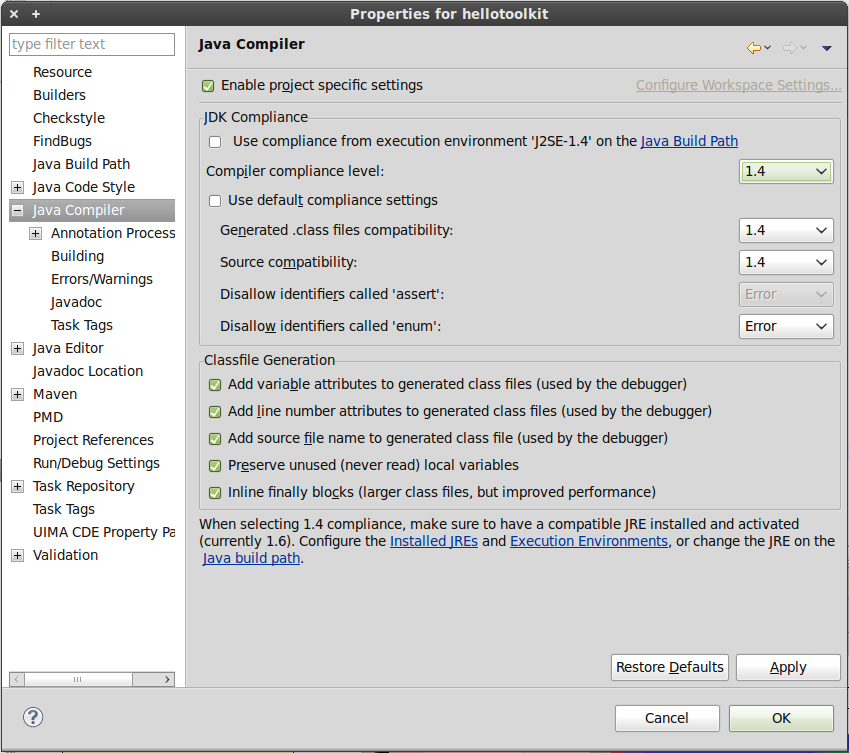
\includegraphics[width=\textwidth]{img/ht08.png}
\caption{Eclipse uses Java 1.4 by default for Maven projects}
\label{fig:java602}
\end{figure}
\begin{figure}
\centering
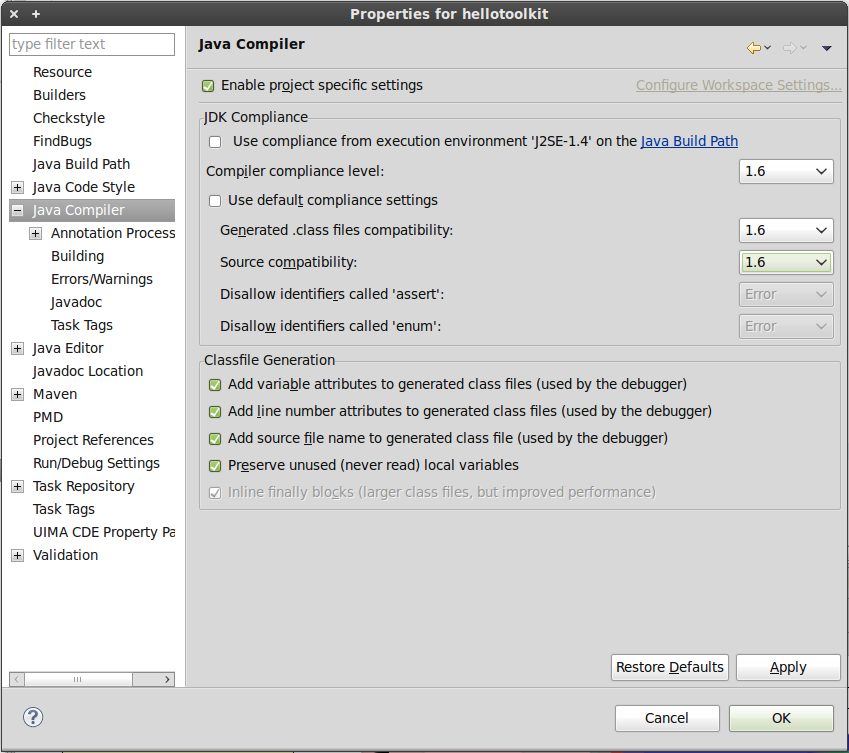
\includegraphics[width=\textwidth]{img/ht09.png}
\caption{Configure Eclipse to use Java 1.6}
\label{fig:java603}
\end{figure}
\begin{figure}
\centering
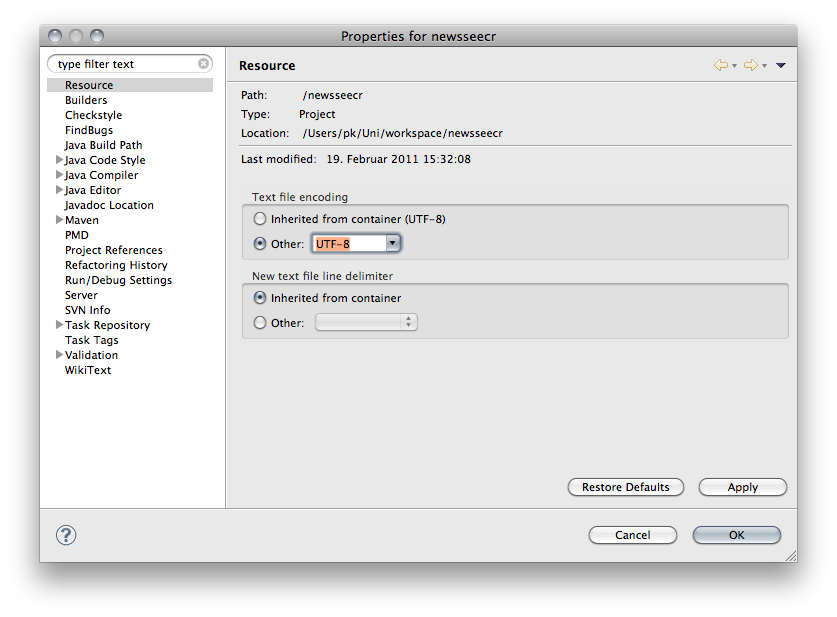
\includegraphics[width=\textwidth]{img/ht16.png}
\caption{Configure Eclipse for UTF-8 encoding}
\label{fig:utf8}
\end{figure}
\paragraph{Writing your first Code with Palladian} Now you can start to write your first code. Your project will already contain the default Maven directory structure. Do not change this structure since Maven depends on it\footnote{Of course you can change Mavens behaviour via the pom.xml but this requires additional configuration not covered by this document. Refer to the Maven documentation under \url{http://maven.apache.org/} for further information.}. As usual we will start with a very simple "Hello World" application. Create a new package \texttt{de.tud.inf.rn.iir.toolkit} and a new class \texttt{HelloToolkit} containing a \texttt{main} method. In this main method you can add actual toolkit code. We used the first example as described in Section~\ref{sec:howto} and search Bing for a string term . The example is also shown in Fig.~\ref{fig:hellotoolkit}.
\begin{figure}
\centering
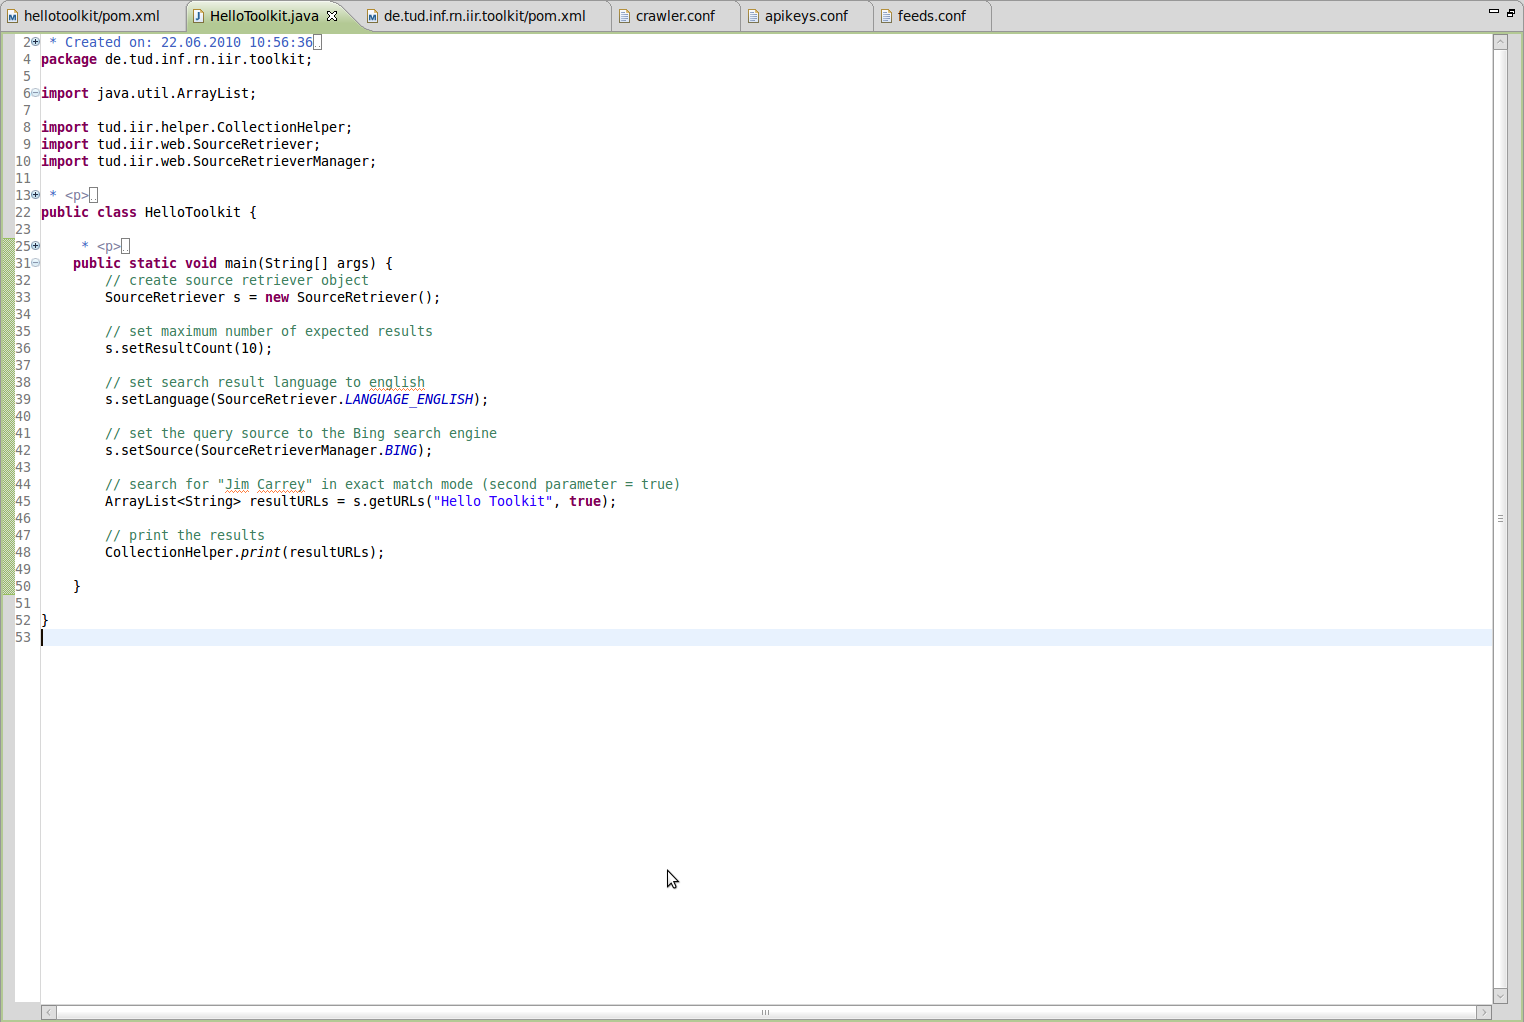
\includegraphics[trim=0 350px 600px 0,clip=true,width=\textwidth]{img/ht10.png}
\caption{"Hello Palladian" Code}
\label{fig:hellotoolkit}
\end{figure}
For the code to work you need copy three files from the config folder in the toolkit project to the config in the source code. These are \texttt{crawler.conf}, \texttt{apikeys.conf} and \texttt{feeds.conf}. You need to copy them to \texttt{src/main/resources/config}. The folder \texttt{src/main/resources} usually contains all resources that are not Java files but are required by your code. All files are shown in Fig.~\ref{fig:resource01}, \ref{fig:resource02} and \ref{fig:resource03}. Fig.~\ref{fig:structure} shows the final directory and file structure of your project.

\begin{figure}
\centering
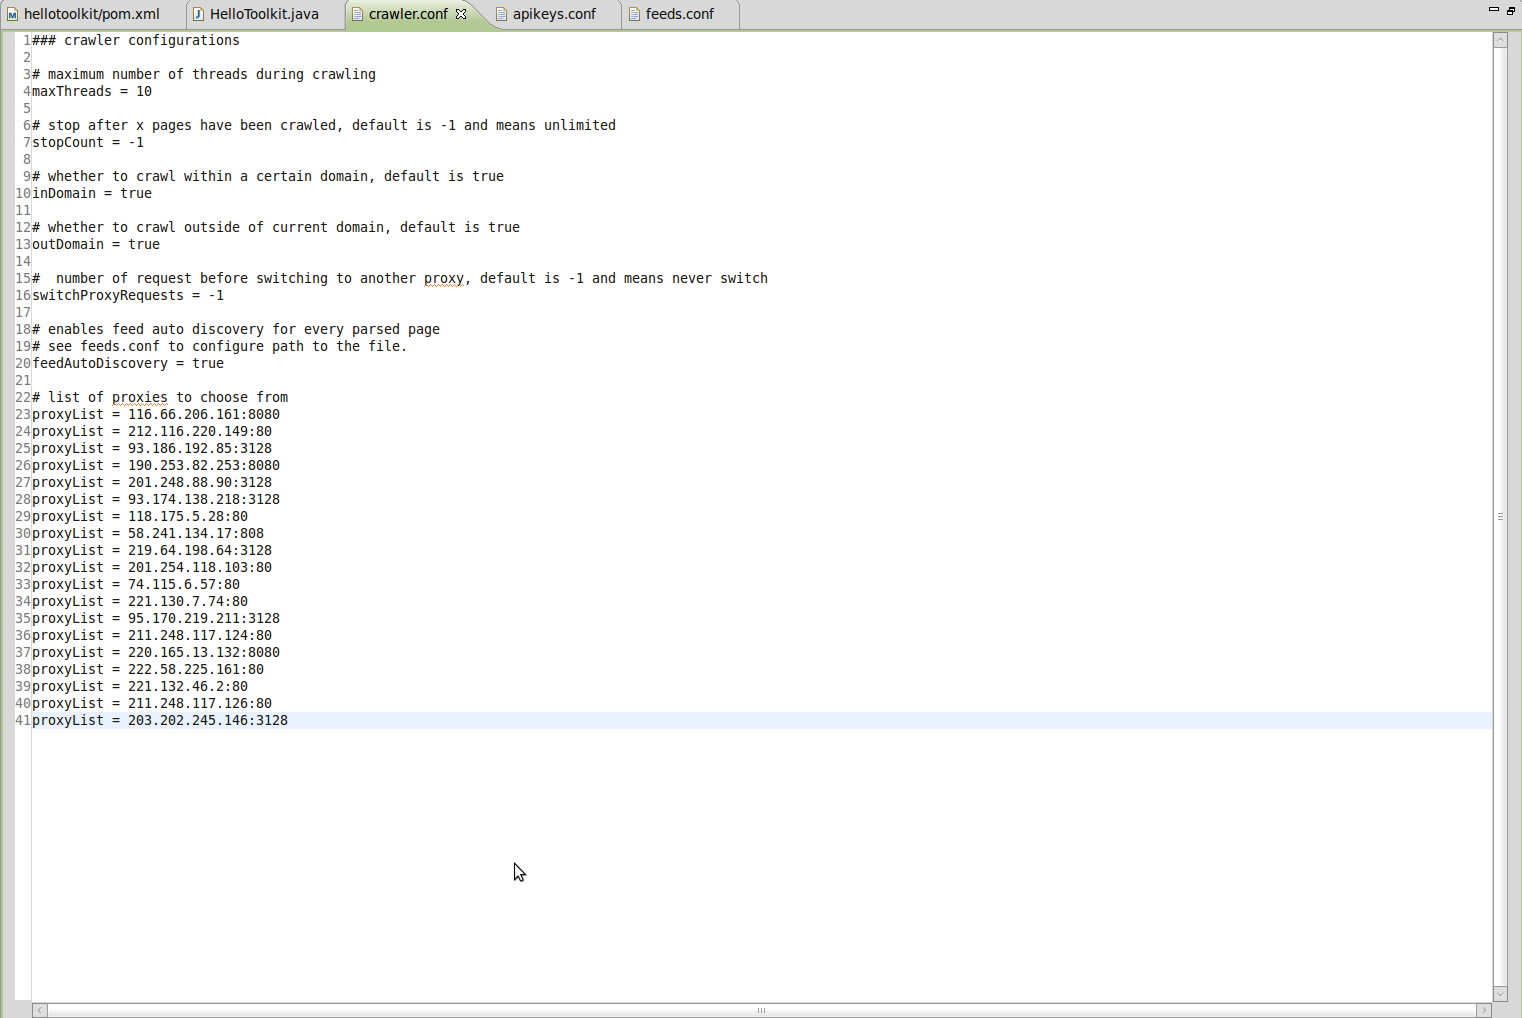
\includegraphics[trim=0 250px 600px 0,clip=true,width=\textwidth]{img/ht11.png}
\caption{\texttt{config/crawler.conf}}
\label{fig:resource01}
\end{figure}
\begin{figure}
\centering
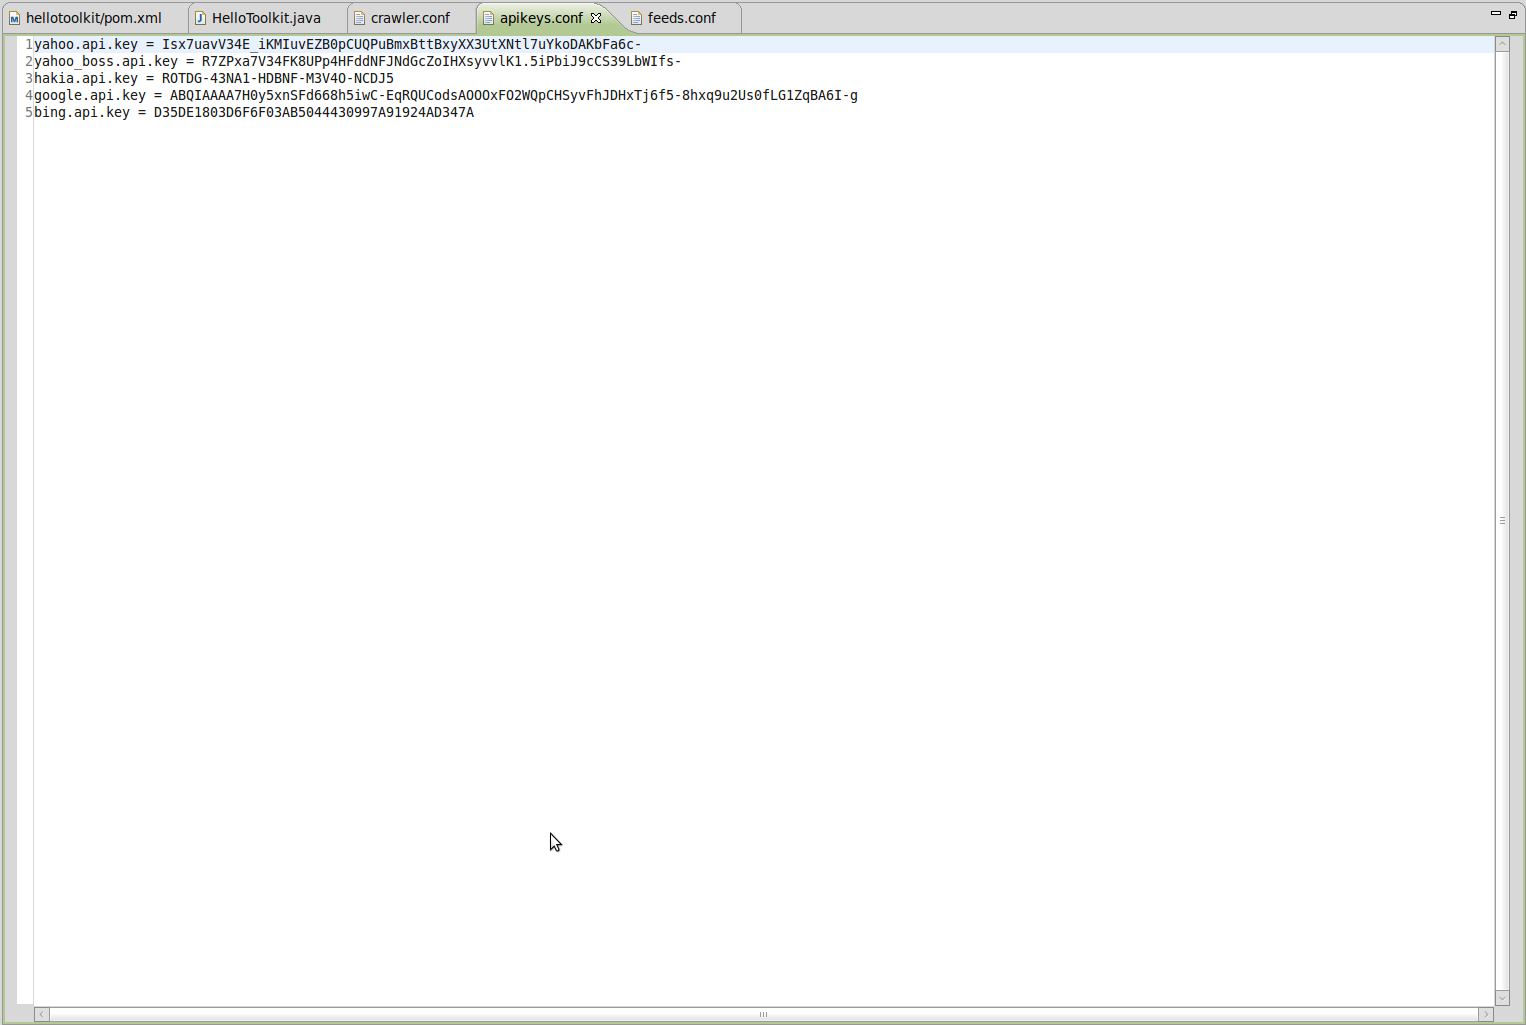
\includegraphics[trim=0 850px 600px 0,clip=true,width=\textwidth]{img/ht12.png}
\caption{\texttt{config/apikeys.conf}}
\label{fig:resource02}
\end{figure}
\begin{figure}
\centering
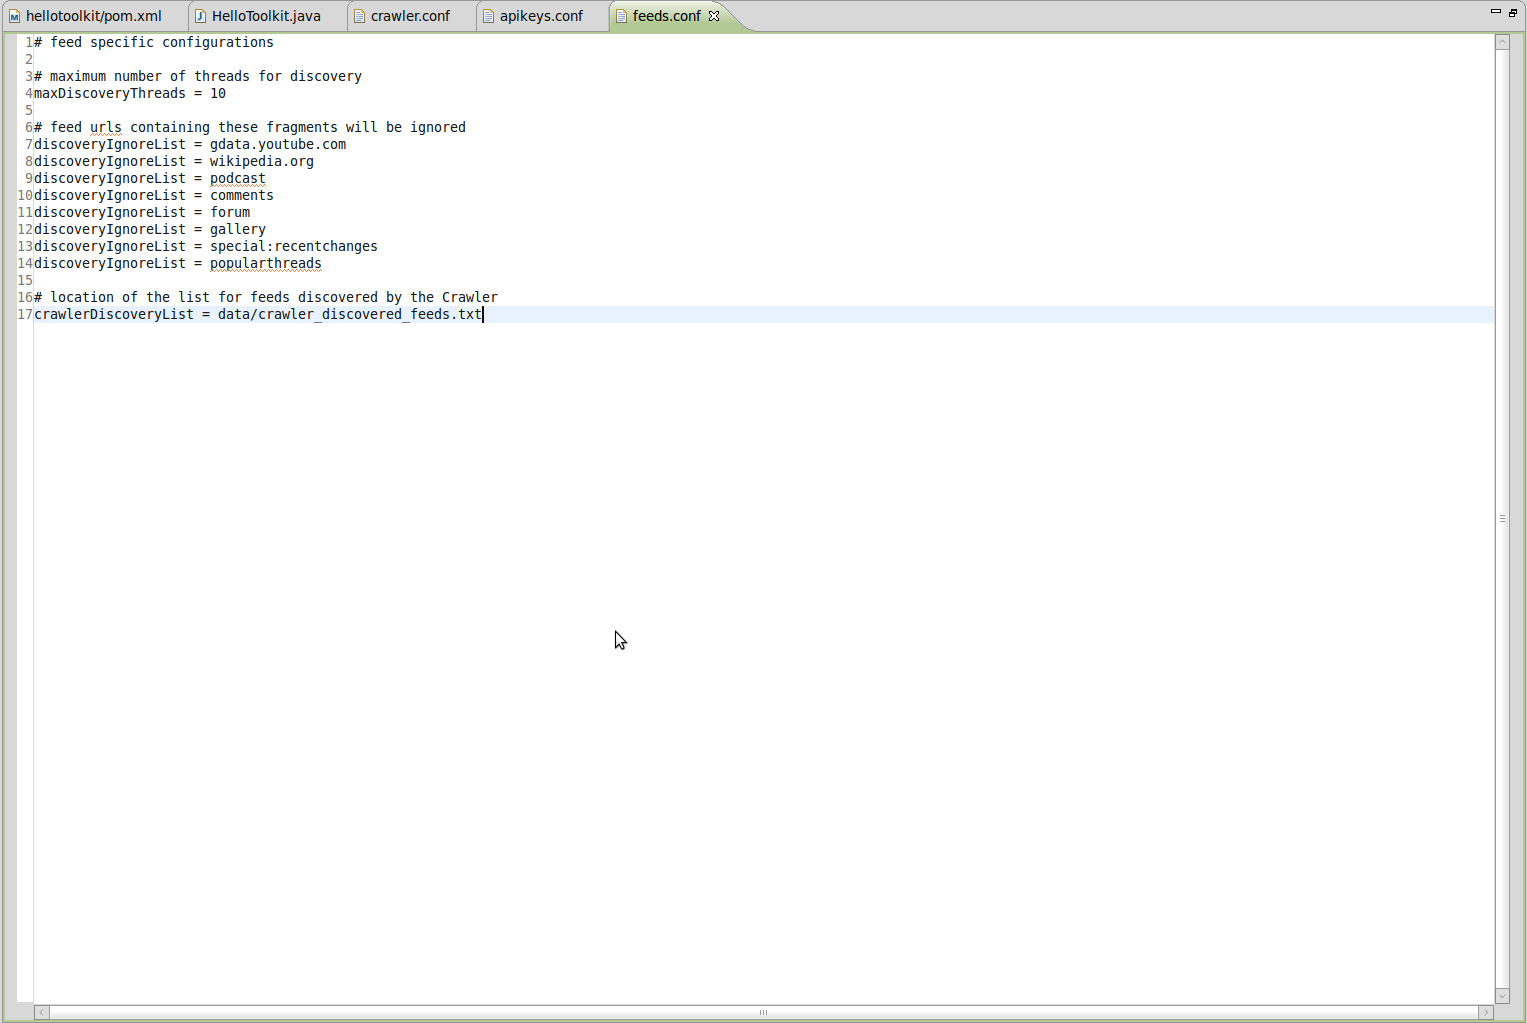
\includegraphics[trim=0 650px 600px 0,clip=true,width=\textwidth]{img/ht13.png}
\caption{\texttt{config/feeds.conf}}
\label{fig:resource03}
\end{figure}
\begin{figure}
\centering
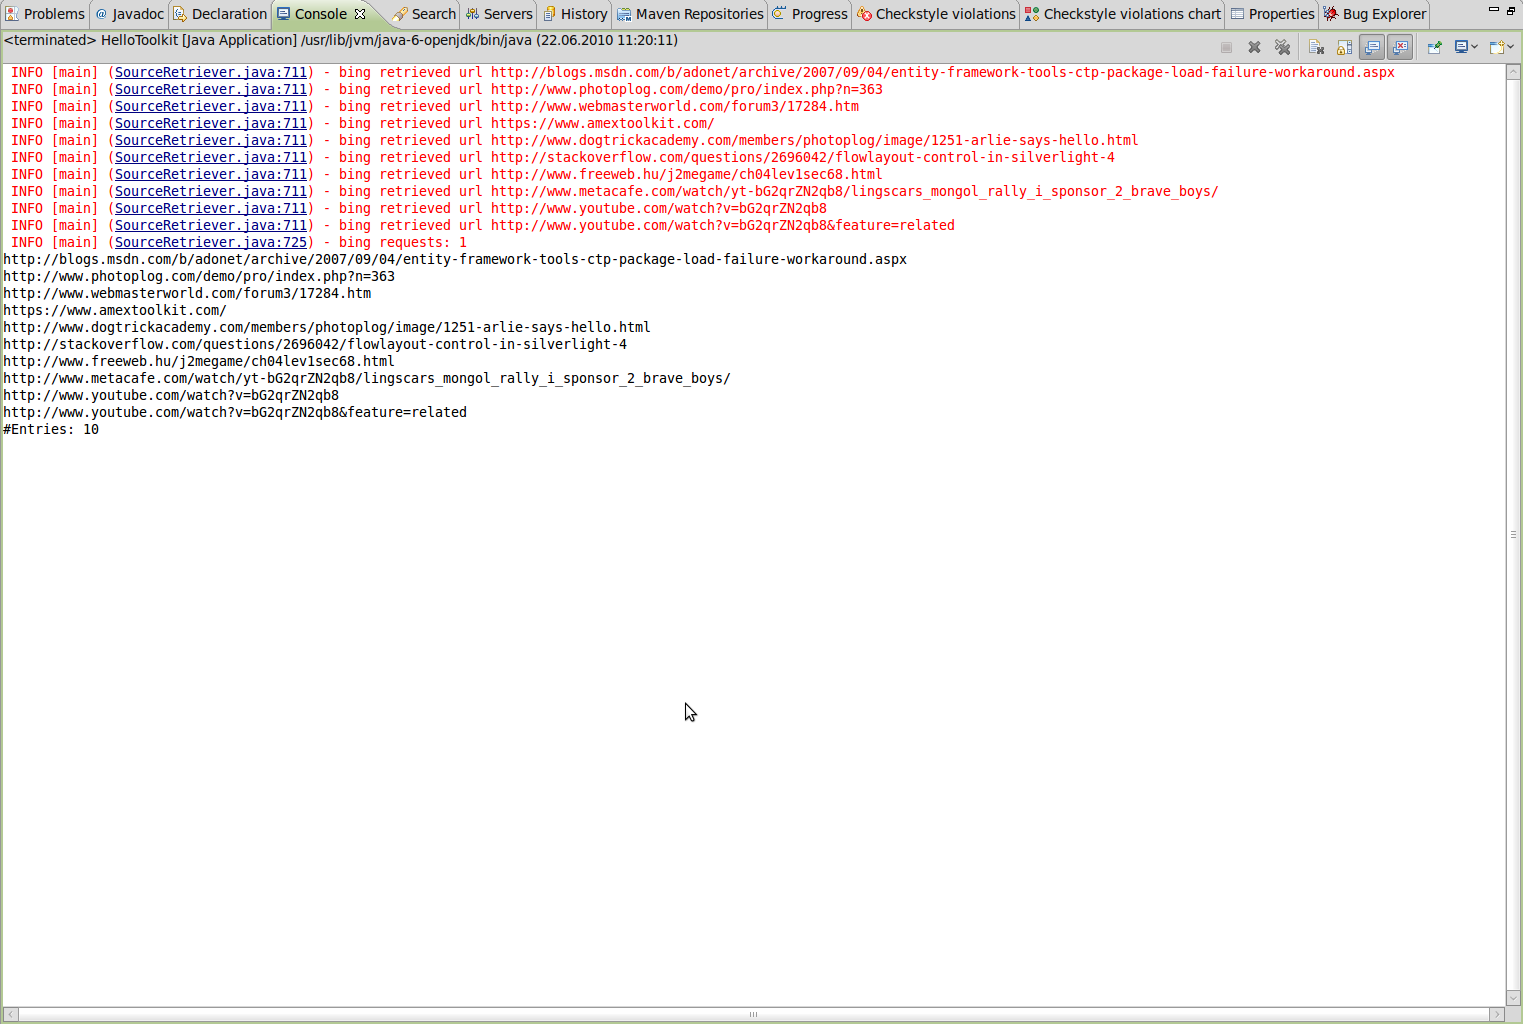
\includegraphics[trim=0 550px 100px 0,clip=true,width=\textwidth]{img/ht14.png}
\caption{"Hello Palladian" Console Output}
\label{fig:structure}
\end{figure}
With the structure from Fig.~\ref{fig:structure} you can run your project. Just open your projects context menu again, choose \textit{Run As $\rightarrow$ Maven Clean}, then open context menu again choose \textit{Run As $\rightarrow$ Maven Install} and finally choose \textit{Run As $\rightarrow$ Java Application}.

\section{Access to Models and Data Sets} \label{sec:AccessModelsDataSets}

Since models and data sets might be very large in file size, they are not included in the SVN repository. As generally no version control is neccessary for this data, we maintain our repository with rsync\footnote{\url{http://rsync.samba.org/}}. rsync is a utility which allows efficient file and directory synchronization between two, local or remote, locations. It was originally developed for Unix systems and should be included with all current Linux distributions and Mac OS X. Altough there are several ports for Windows systems, we recommend using the cwrsync\footnote{\url{http://www.itefix.no/i2/node/10650}} package. 

Palladian comes with convenient ready-to-use scripts to download models and data sets from our central repository. The scripts are called \texttt{dataSync.bat} for Windows and \texttt{dataSync.sh} for Linux and Mac OS X and can be found in the \texttt{dev} directory. Make sure to set the \texttt{DESTINATION} variable inside the script before initial usage. On Windows operating systems, you further need to add the directory with the rsync binaries to your \texttt{PATH} environment variable, which can be done using the ``System Properties'' control panel (See Fig.~\ref{fig:rSyncWindowsPath1} and ~\ref{fig:rSyncWindowsPath2}).

Please contact the toolkit managers if you need write access to the rsync repository.


\begin{figure}
\centering
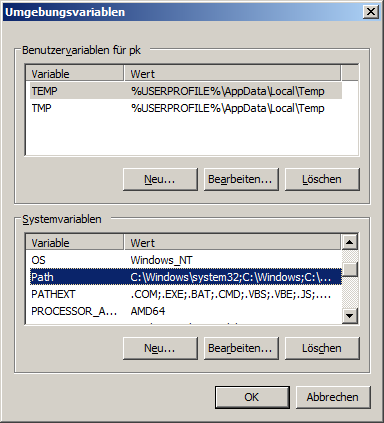
\includegraphics[scale=0.8]{img/WindowsPath1.png}
\caption{Configuring PATH on Windows}
\label{fig:rSyncWindowsPath1}
\end{figure}

\begin{figure}
\centering
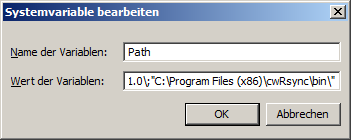
\includegraphics[scale=0.8]{img/WindowsPath2.png}
\caption{Configuring PATH on Windows}
\label{fig:rSyncWindowsPath2}
\end{figure}


\section{Reporting Issues using Redmine}
To report issues with the toolkit or to view issues assigned to you, you need to register to Redmine. To do this send an E-Mail to the administrator at \href{mailto:klemens.muthmann@tu-dresden.de}{klemens.muthmann@tu-dresden.de} and provide your name, your advisor, and the reason why you are working on Palladian (i.e. thesis topic or research fellow). You will receive an E-Mail (not automatically so it might take some time) providing a link where you can set your password. If you successfully set a password for your account you can login on: \href{http://redmine.effingo.de/}{Redmine}.
%\subsection{Building the toolkit using Apache Ant}
%You can also build the toolkit using Apache Ant\footnote{\url{http://ant.apache.org/}}. To do so, install Apache Ant, put the binary folder to your PATH and compile the project from the root folder that contains the build.xml file.
%The following tasks can be performed by ant (type commands into your console):
%\begin{itemize}
%\item \textbf{standard} Type ``ant'' to clean and compile the project.
%\item \textbf{jar} Type ``ant jar'' to pack TUDIIR into one single jar file. That file can then be found under target/jar/tudiir.jar.
%\item \textbf{javadoc} Type ``ant javadoc'' to (re)create the javadoc which can then be found under documentation/javadoc. You  need to install Graphviz\footnote{\url{http://www.graphviz.org/}} beforehand. See Java Dzone\footnote{\url{http://java.dzone.com/articles/reverse-engineer-source-code-u}} for more information.
%\end{itemize}
%Apache Ant will create a target folder, please do not commit that folder to the repository but ignore it using svn:ignore.

\chapter{Toolkit Structure}
\label{sec:toolkitstructure}
TUD Palladian is managed using subversion. The top level folder structure follows the usual subversion layout using trunk for the main development, branches for parallel development and tags to mark specific versions. The trunk is located in our SVN\footnote{\url{https://141.76.40.86/svn-students/iircommon/toolkit/trunk}}. The folder structure looks as follows.
\begin{verbatim}
palladian
 |- config
 |- data
    |- datasets
    |- knowledgeBase
    |- models
    |- test
 |- documentation
    |- handout
    |- javadoc
 |- exe
 |- src
    |- main
       |- java
    |- test
       |- java
 |- dev
\end{verbatim}

\section{Config Folder}

% TODO this needs to be adapted to the new single config file ...

\label{sec:config.conf}
The config folder contains configuration files for several components of the toolkit. The files are explained in the following sections.

\subsection{apikeys.conf}
\label{sec:apikeys.conf}
The api keys that are used by the toolkit components are specified here. You may need to apply for API keys at the provider's page.

\begin{verbatim}
yahoo.api.key = 
yahoo_boss.api.key = 
hakia.api.key = 
google.api.key = 
bing.api.key = 
\end{verbatim}

\subsection{classification.conf}
\label{sec:classification.conf}
Classification settings for the ws.palladian.classification.page.ClassifierManager.

\begin{verbatim}
# percentage of the training/testing file to use as training data
page.trainingPercentage = 80

# create dictionary on the fly (lowers memory consumption but is slower)
page.createDictionaryIteratively = false

# alternative algorithm for n-gram finding (lowers memory consumption but is slower)
page.createDictionaryNGramSearchMode = true

# index type of the classifier:
# 1: use database with single table (fast but not normalized and more disk space needed)
# 2: use database with 3 tables (normalized and less disk space needed but slightly slower)
# 3: use lucene index on disk (slow)
page.dictionaryClassifierIndexType = 1
\end{verbatim}

\subsection{crawler.conf}
\label{sec:crawler.conf}
Crawler settings for the ws.palladian.web.Crawler. All settings can be set in Java code as well.

\begin{verbatim}
# maximum number of threads during crawling
maxThreads = 10

# stop after x pages have been crawled, default is -1 and means unlimited
stopCount = -1

# whether to crawl within a certain domain, default is true
inDomain = true
	
# whether to crawl outside of current domain, default is true
outDomain = true

#  number of request before switching to another proxy, default is -1 and means never switch
switchProxyRequests = -1
	
# list of proxies to choose from
proxyList = 83.244.106.73:8080
proxyList = 83.244.106.73:80
proxyList = 67.159.31.22:8080
\end{verbatim}

\subsection{db.conf}
Database settings for the ws.palladian.persistence.DatabaseManager.

\begin{verbatim}
db.type = mysql
db.driver = com.mysql.jdbc.Driver
db.host = localhost
db.port = 3306
db.name = toolkitdb
db.username = root
db.password = rootpass
\end{verbatim}

\subsection{general.conf}
General settings used by the ws.palladian.control.Controller.

\section{Data Folder}
The data folder contains files that are used during runtime of several components.

\subsection{knowledgeBase} 
The knowledge base folder contains the OWL ontology files used for the extraction tasks in the ws.palladian.extraction package.

\subsection{models}
The models folder contains learned models that can be reused. See section \ref{sec:AccessModelsDataSets} for an explanation on how to access our extensive collection of data sets and models.

\subsection{Temp Folder}
The temp folder is not part of the repository. Some functions may however create this folder and write temporary data.

\subsection{test}  
The test folder contains data that is used for running jUnit tests.

\section{Documentation Folder}
The documentation folder contains help files to understand the toolkit. This very document is located in the handout folder and a Javadoc can be found there too.

\section{Exe Folder}
The exe folder contains all runnable jar files in separate folders including a sample script to run the program and a readme.txt that explains the run options.

\section{Libs Folder}
The libs folder contains all referenced libs used by the toolkit.

\section{Src Folder}
The src folder contains all source files of the toolkit. You may need to put the log4j.properties file here in order to use custom logging settings. Alternatively you include the config folder in the class path.


\chapter{Conventions}
\section{Coding Standards}
To keep the code readable and easy to understand for other developers, we use the following coding guidelines.
%http://geosoft.no/development/javastyle.html
\begin{enumerate}
\item All text is written in (American) English (color instead of colour).
\item Variables and method names should be camel cased and not abbreviated ($computeAverage$ instead of $comp\_avg$).
\item There must be a space after a comma.
\item There must be a line break after opening $\{$ braces.
\item Static fields must be all uppercase. There should be an $\_$ for longer names ($STATIC\_FIELD$).
\item Each class must have a comment including the author name.
\item Methods with very simple, short code do not need to have comments (getters and setters) all other methods should have an explaining comment with @param explanation and @return.
\item Avoid assignments ($=$) inside if and while conditions.
\item Statements after conditions should always be in braces ($\{\}$)
\end{enumerate}

Listing~\ref{lst:CodingStandards} shows an example class with applied coding standards. Please also have a look at \cite{codingStandards} for a quick overview of best practices.

\begin{codelisting}
\begin{lstlisting}[caption=Example class for coding guidelines,label=lst:CodingStandards,frame=tb]
/**
 * This is just an example class.
 * It is here to show the coding guidelines.
 * 
 * @author Forename Name
 */
public class ExampleClass implements Example {

	// this field holds all kinds of brackets
	private static final char[] BRACKET_LIST = {'(', ')'};

	/**
	 * This is just and example method.
	 * 
	 * @param timeString A string with a time.
	 * @return True if no error occurred, false otherwise.
	 */
	public boolean computeAverageTime(String timeString) {
		if (hours < 24 && minutes < 60 && seconds < 60) {
			return true;
		} else {
			return false;
		}
	}
}
\end{lstlisting}
\end{codelisting}

\section{Eclipse Plugins for better Coding}
\label{sec:eclipseCodingPlugins}
It is a very good practice to install the following eclipse plugins to check ones own code before committing:
\begin{enumerate}
\item CodeFormatter is a simple file that can be loaded into Eclipse to format the source code correctly. Go to Eclipse $\blacktriangleright$ Window $\blacktriangleright$ Preferences $\blacktriangleright$ Java $\blacktriangleright$ Code Style $\blacktriangleright$ Formatter and import the ``tudiir\_eclipse\_formatter.xml'' from the dev folder. Pressing Control+F formats the source code of a selected class.
\item Checkstyle \footnote{\url{http://eclipse-cs.sourceforge.net/downloads.html}} checks styles of the code, whether JavaDoc comments are set etc. After installing you should go to the preferences section of Checkstyle in Enclipse and load the ``checkstyle\_config.xml'' from the dev folder.
\item PMD\footnote{\url{http://pmd.sourceforge.net/eclipse/}} tells you what is wrong with your code in terms of common violations, forgotten initializations and much more. After installing you should go into the preferences of PMD and load the ruleset file ``pmd\_ruleset'' from the dev folder.
\item FindBugs\footnote{\url{http://findbugs.cs.umd.edu/eclipse/}} is similar to PMD but focuses on severe errors only. After installing you don't need to configure anything.
\end{enumerate}

Checkstyle, PMD, and FindBugs can be initiated by right clicking a package or class file and selecting the plugin. The violations will be shown so that you can eliminate them.

Using these plugins raises the chances to win in the continuous integration game as described in Section \ref{sec:cigame}.

\subsection{Tests}
To guarantee that all components work as expected, we use jUnit tests. Before major check-ins to the repository, all jUnit Tests must run successfully. Run the ws.palladian.control.AllTests.java to make sure all components work correctly.
After finishing a new component, new testing code must be written.

%\section{Project Management}
\chapter{Toolkit Functionality}
In this chapter we discuss the functionalities of Palladian in detail. The purpose of each section is to give a general understanding of how the algorithms work and how to use them practically.

\section{Classification}

\subsection{Text Classification}
Text classification is the process of assigning one or more categories to a given text document. There are several types of text classification which are shown in Figure \ref{fig:typesOfClassification}. Palladian can classify text in a single category, multiple categories, or in a hierarchical manner.

\begin{figure}[ht!]
\centering
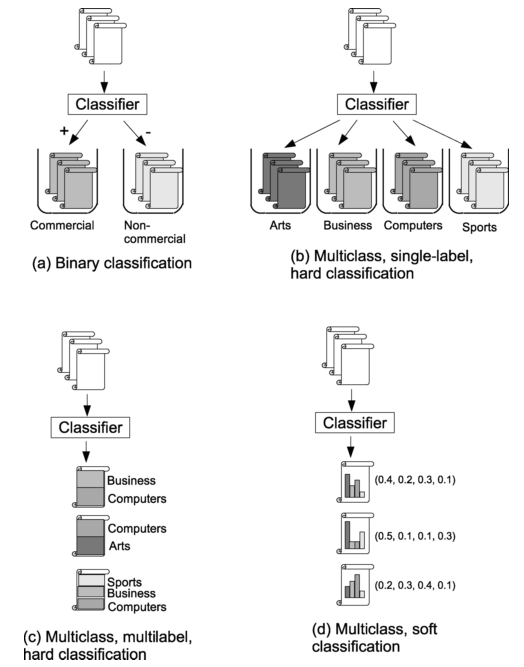
\includegraphics[width=4in]{img/typesOfClassification.png}
\caption{Types of classification\cite{qi2009web}.}
\label{fig:typesOfClassification}
\end{figure}

The text classification components are built from scratch and do not rely on external libraries such as Weka. In this section we will explain which features can be used for the classification, the basic theory of the classifiers, and how the performance of a classifier can be evaluated. In each section, we will describe theory and how the classification components can be used programmatically.

\subsubsection{Classification Type}
Palladian supports simple single category classification, tagging, and hierarchical classification. Each classifier needs to know in which type it has to perform classification.
This information is stored in the ClassificationTypeSetting object which is then passed to the classifier. Please read the Javadoc of that class for more detailed information.

\subsubsection{Features}
Features are the input for a classifier. In text classification we have a long string as an input from which we can derive several features. All of Palladian's classifiers work with n-grams. N-grams are sets of tokens of the length n. Palladian can preprocess text with character or word-level n-grams. See Section \ref{sec:ngrams} for more details.

Sometimes you do not want to have all n-grams to be features for the classifier. You can simply disallow certain features by putting them in a stop word list. These n-grams will then be ignored for the classification.

%CODE
All these settings are stored in a FeatureSetting object which is passed to the classifier. Please read the Javadoc of that class for more detailed information.

\subsubsection{Text Classifiers}
The text classifiers perform the actual classification task by calculating the most relevant category (or categories) for the input document. Two text classifiers are implemented, a dictionary based classifier and a k-nearest neighbor classifier. Both are explained in more detail in the following paragraphs.

\paragraph{K-Nearest Neighbor Text Classifier}
The KNN classifier uses the n-grams of the training documents to place them in a high dimensional vector space. The dimensions of the space equal the total number of available n-grams. Each training document is therefore a vector in that highly dimensional space. A new, unclassified document is now put into that vector space and by using distance function the k nearest neighbors are found for that document. Each of these neighbors votes with its own class, the more votes for one class the more likely that the new document belongs to that class.

\begin{figure}[ht!]
\centering
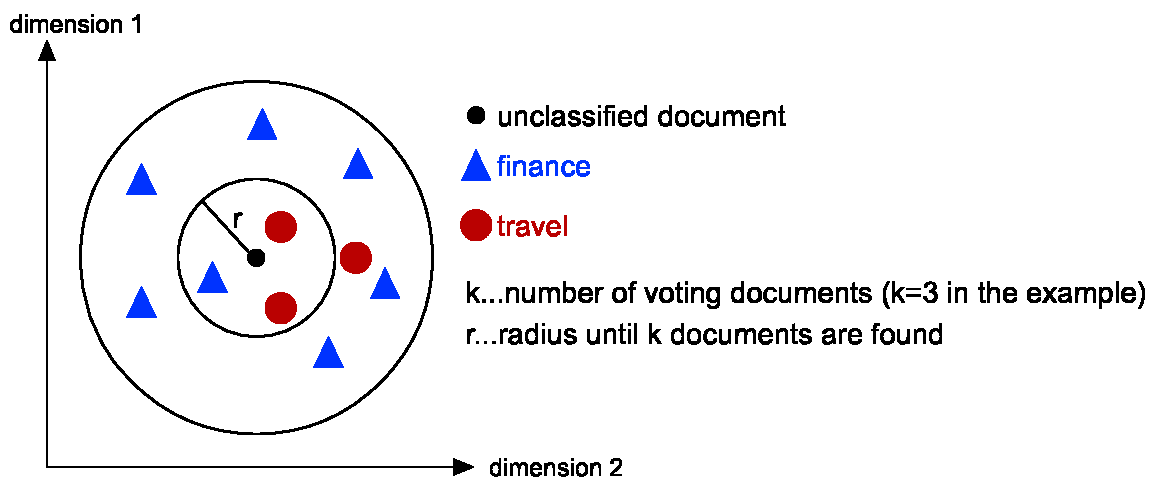
\includegraphics[width=0.8\textwidth]{img/knn.pdf}
\caption{A simple KNN example.}
\label{fig:knn}
\end{figure}

Figure \ref{fig:knn} shows a simple example of how the KNN classifier works. We limited the dimension to two for easier understanding. In this scenario we want to classify the given document (black dot in the middle) into one of the two categories ``finance'' (blue triangles) or ``travel'' (red dots). We calculate the distance between the new document and all training documents and consider the votes of the nearest three. In the example, two of these three document vote for ``travel'' which would let us classify our input document into that class.

The distance between two documents is calculated as shown in Equation \ref{eqn:knnDistance} where $d1$ and $d2$ are the two documents. The shorter the distance, the more similar the documents.

\begin{equation}
\label{eqn:knnDistance}
distance(d1,d2) = \frac{1}{numberOfMatchingNGrams}
\end{equation}

\paragraph{Dictionary-Based Classifier}
The dictionary-based classifier\footnote{This classifier won the first Research Garden (\url{http://www.research-garden.de}) competition where the goal was to classify product descriptions into 8 different categories. See press release at \url{http://www.research-garden.de/c/document_library/get_file?uuid=e60fa8da-4f76-4e64-a692-f74d5ffcf475&groupId=10137}} learns how probable each n-gram is for each given category and assigns the most probable category (or categories) to the input document.

A dictionary is built at training stage by counting and normalizing the co-occurrences of one n-gram and a category. The dictionary might then look as shown in Table \ref{tab:dictionary} where each column is a category (finance, travel, and science) and each row is an n-gram. In each cell we now have the learned relevance for each n-gram and category $relevance(ngram,category)$. The sum of the relevances in each row must add up to one.

Table \ref{tab:dictionary} shows an example dictionary matrix. The n-gram ``money'' is more likely to get the category ``finance'' ($relevance(money,finance) = 0.6$) than ``science'' ($relevance(money,science) = 0.25$) while the n-gram ``beach'' is most likely to appear in the category ``travel'' ($relevance(beach,travel) = 0.85$.

\begin{table}[ht]
\centering
\begin{tabular}{|l|l|l|l|}
\hline
n-gram   & finance & travel & science \\
\hline
money	   & 0.6	&	0.15	&	0.25	\\
\hline
beach	& 0.1	&	0.85	&	0.05	\\
\hline
paper	   & 0.3 &	0.2	&	0.5	\\
\hline
\end{tabular} 
\caption{N-Gram dictionary with relevances for categories.}
\label{tab:dictionary}
\end{table}

To classify a new document, we again create all n-grams, look up the relevance scores in the dictionary and assign the categories with the highest probability. The probability for each category and given document is calculated as shown in Equation \ref{eqn:dictionaryCategoryProbabilty} where $N_{Document}$ is the set of n-grams for the given document.

\begin{equation}
\label{eqn:dictionaryCategoryProbabilty}
\mbox{$CategoryProbability(category,document)$} = \sum_{n\,\epsilon\, Nurl} \mbox{$relevance(n,category)$}
\end{equation}

The dictionary can be stored in memory, in an embedded H2 database, or in a client/server MySQL database. These settings can be made in the classification.conf file in the conf folder (see Section \ref{sec:config.conf}).

%TODO category boost
%TODO cooccurrence

\subsubsection{Evaluation}
In order to find out which classifier works best with which feature settings, you can evaluate these combinations. The ws.palladian.classification.page.ClassifierManager has the $learnBestClassifier$ method to run the evaluation on all given classifiers with the given evaluation setting object ws.palladian.classification.page.EvaluationSetting. See Section \ref{sec:bpTextClassification} for more details of how to perform the evaluation programmatically.

The output of the evaluation will be three csv files that hold information about the combinations of classifier, dataset, training percentage, and the final performance for the combination. The performance is measured in precision, recall, and F1. The three files are stored in the data/temp folder and hold the following information.

\paragraph{averagePerformancesDatasetTrainingFolds.csv} This file holds the performance measures for each classifier, averaged over all given datasets, training percentages, and folds in the cross validation.

\paragraph{averagePerformancesTrainingFolds.csv} This file holds the performance measures for each classifier and dataset combination, averaged over all given training percentages and folds in the cross validation.

\paragraph{averagePerformancesFolds.csv} This file holds the performance measures for each classifier, dataset, and training percentage combination, averaged over all given folds in the cross validation.

\subsubsection{Best Practices}
\label{sec:bpTextClassification}
This section describes how to prepare training and testing data to learn a model, evaluate, and use a text classifier.

\paragraph{Preparing the Training/Testing Data}
The data can be specified in a simple text file. There are three classification options, namely, one-category classification, hierarchical classification and multi-category classification. They all require a similar structure of the data.

\subparagraph{One-Category Classification}
We write one URL and one category separated with a single space on each line. For example:
\begin{verbatim}
http://www.google.com search
http://www.fifa.com sport
http://www.oscars.com entertainment
\end{verbatim}

\subparagraph{Hierarchical Classification}
We write one URL and multiple categories separated with a single space on each line. The categories must be in the correct order, so the first category is the main one, all following are subcategories of each other. For example:
\begin{verbatim}
http://www.google.com search search_engine
http://www.fifa.com sport team_sports soccer 
http://www.oscars.com entertainment movies awards usa
\end{verbatim}

\subparagraph{Multi-Category Classification}
We write one URL and multiple categories separated with a single space on each line. The order of the categories (tags) does not matter. For example:
\begin{verbatim}
http://www.google.com search image_search video_search
http://www.fifa.com soccer sport free_time fun ball_game results to_read
http://www.oscars.com entertainment movies films awards watch video stars
\end{verbatim}

\paragraph{Training a classifier}
Before we can use a classifier, we need to learn a model. The model is an internal representation of the learned data. After learning a model, a classifier can applied to unseen data. We now have prepared the training and testing data so we can now learn the models.
The classifier is saved as a lucene index or a database under the name of the classifier with a ``Dictionary'' suffix. The result of the learning are three files: the classifier (``CLASSIFIER.ser''), the dictionary object (``CLASSIFIERDictionary.ser''), and the actual dictionary as the index or database (e.g. ``CLASSIFIERDictionary.h2.db''). More settings can be configured in the config/classification.conf file. See \ref{sec:classification.conf} for more information.

Listing \ref{listing:trainClassifier} shows an example for how to train and save a classifier. In this case we train a classifier that can classify the language of given documents. As training data we use a list of web pages of different languages from Wikipedia.

\begin{codelisting}
\begin{lstlisting}[label=listing:trainClassifier,caption=Training a classifier.,frame=tb]
// create a classifier mananger object
ClassifierManager classifierManager = new ClassifierManager();

// specify the dataset that should be used as training data
Dataset dataset = new Dataset();

// set the path to the dataset
String dsPath = "data/datasets/classification/language/index.txt";
dataset.setPath(dsPath);

// tell the preprocessor that the first field in the file is a link to 
// the actual document
dataset.setFirstFieldLink(true);

// create a text classifier by giving a name and a path 
// where it should be saved to
String dcn = "LanguageClassifier";
String dcp = "data/models/languageClassifier/";
TextClassifier classifier = new DictionaryClassifier(dcn,dcp);

// specify the settings for the classification
ClassificationTypeSetting cts = new ClassificationTypeSetting();

// we use only a single category per document
cts.setClassificationType(ClassificationTypeSetting.SINGLE);

// we want the classifier to be serialized in the end
cts.setSerializeClassifier(true);

// specify feature settings that should be used by the classifier
FeatureSetting featureSetting = new FeatureSetting();

// we want to create character-level n-grams
featureSetting.setTextFeatureType(FeatureSetting.CHAR_NGRAMS);

// the minimum length of our n-grams should be 3
featureSetting.setMinNGramLength(3);

// the maximum length of our n-grams should be 5
featureSetting.setMaxNGramLength(5);

// we assign the settings to our classifier
classifier.setClassificationTypeSetting(classificationTypeSetting);
classifier.setFeatureSetting(featureSetting);

// now we can train the classifier using the given dataset
classifierManager.trainClassifier(dataset, classifier);
\end{lstlisting}
\end{codelisting}

\paragraph{Using a classifier}
After we trained a model for a classifier we can apply it to unseen data. Let's use the model we just trained to classify the language of a new document.

Listing \ref{listing:useClassifier} shows how to use a trained classifier.

\begin{codelisting}
\begin{lstlisting}[label=listing:useClassifier,caption=Use a trained text classifier.,frame=tb]
// the path to the classifier we want to use
String path = "data/models/languageClassifier/LanguageClassifier.ser";

// load the language classifier
TextClassifier classifier = ClassifierManager.load(path);

// create a classification document that holds the result
ClassificationDocument classifiedDocument = null;

// classify the little text (if classifier works it would say Spanish)
classifiedDocument = classifier.classify("Yo solo s� que no s� nada.");

// print the classified document
System.out.println(classifiedDocument);
\end{lstlisting}
\end{codelisting}

You can also try the language classifier online at \url{http://www.webknox.com/wi#detectLanguage}.

\paragraph{Evaluating a Classifier}
To get an idea of how good a trained classifier works, we can evaluate it using test data which is structured the same way as the training data. Listing~\ref{listing:evaluateClassifier} shows how to evaluate a trained classifier, you will see that is very similar to training a classifier. Make sure that you evaluate the classifier using disjunct data, otherwise the evaluation results are invalid .

\begin{codelisting}
\begin{lstlisting}[label=listing:evaluateClassifier,caption=Evaluating a trained text classifier.,frame=tb]
// create a classifier mananger object
ClassifierManager classifierManager = new ClassifierManager();

// the path to the classifier we want to use
String path = "data/models/languageClassifier/LanguageClassifier.ser";

// specify the dataset that should be used as testing data
Dataset dataset = new Dataset();

// the path to the dataset (should NOT overlap with the training set)
dataset.setPath("data/datasets/classification/language/index.txt");

// tell the preprocessor that the first field in the file is a link
// to the actual document
dataset.setFirstFieldLink(true);

// load the language classifier
TextClassifier classifier = ClassifierManager.load(path);

// now we can test the classifier using the given dataset
ClassifierPerformance classifierPerformance = null;
classifierManager.testClassifier(dataset, classifier);
\end{lstlisting}
\end{codelisting}

\paragraph{Testing parameter combinations}
As you have seen, you can train the classifier using different parameters. So how can you be sure that you set the parameters correctly? Do they work well on different datasets? Is the chosen classifier always better than others? In order to answer these questions with hard data you can automatically run different combinations of classifiers, settings, and datasets as shown in Figure \ref{fig:bcc}. The green line shows the combination that was found to perform best. In the end you will get one evaluation csv with information about how the combination performed. You can then manually pick the best performing settings.

\begin{figure}[ht!]
\centering
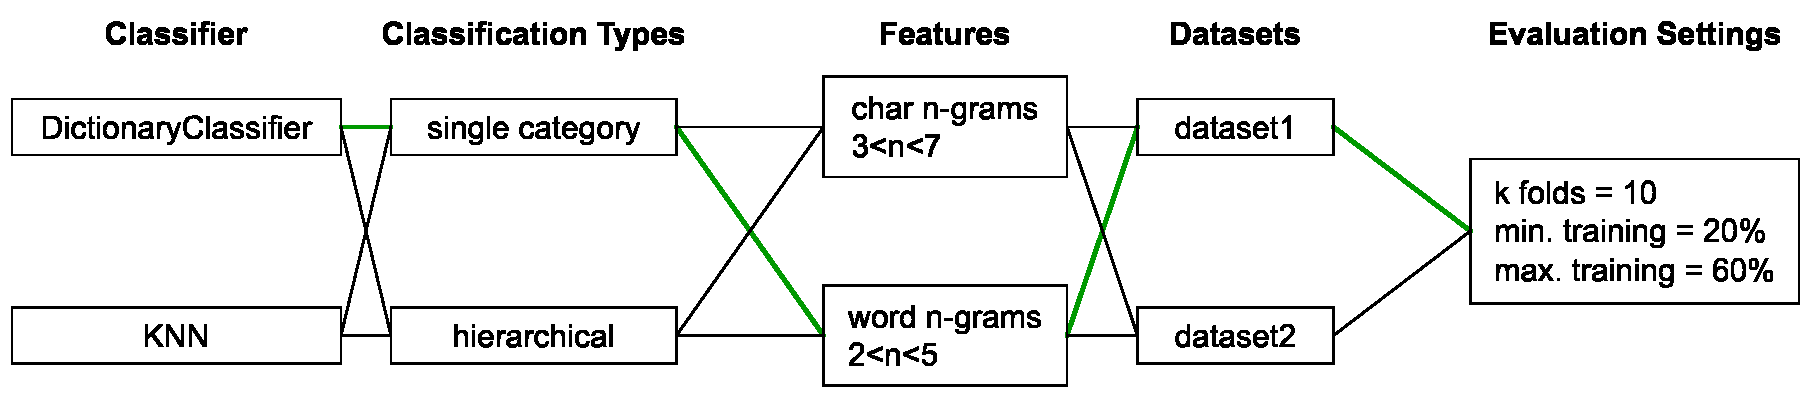
\includegraphics[width=\columnwidth]{img/bcc.pdf}
\caption{Combinations for training a solid classifier.}
\label{fig:bcc}
\end{figure}

Listing \ref{listing:bcc} shows you how to do just that.

\begin{codelisting}
\begin{lstlisting}[label=listing:bcc,caption=Learning the best parameter combination for a text classifier.,frame=tb]
ClassifierManager classifierManager = new ClassifierManager();

// build a set of classification type settings to evaluate
List<ClassificationTypeSetting> ctsList;
ctsList = new ArrayList<ClassificationTypeSetting>();
ClassificationTypeSetting cts = new ClassificationTypeSetting();
cts.setClassificationType(ClassificationTypeSetting.SINGLE);
cts.setSerializeClassifier(false);
ctsList.add(cts);

// build a set of classifiers to evaluate
List<TextClassifier> classifiers = new ArrayList<TextClassifier>();
TextClassifier classifier = null;
classifier = new DictionaryClassifier();
classifiers.add(classifier);
classifier = new KNNClassifier();
classifiers.add(classifier);

// build a set of feature settings for evaluation
List<FeatureSetting> featureSettings = new ArrayList<FeatureSetting>();
FeatureSetting fs = null;
fs = new FeatureSetting();
fs.setTextFeatureType(FeatureSetting.CHAR_NGRAMS);
fs.setMinNGramLength(3);
fs.setMaxNGramLength(7);
featureSettings.add(fs);

fs = new FeatureSetting();
fs.setTextFeatureType(FeatureSetting.CHAR_NGRAMS);
fs.setMinNGramLength(2);
fs.setMaxNGramLength(5);
featureSettings.add(fs);

fs = new FeatureSetting();
fs.setTextFeatureType(FeatureSetting.WORD_NGRAMS);
fs.setMinNGramLength(2);
fs.setMaxNGramLength(5);
featureSettings.add(fs);

// build a set of datasets that should be used for evaluation
Set<Dataset> datasets = new HashSet<Dataset>();
Dataset dataset = new Dataset();
dataset.setPath("dataset1.txt");
datasets.add(dataset);
dataset = new Dataset();
dataset.setPath("dataset2.txt");
dataset.setSeparationString("#");
datasets.add(dataset);

// set evaluation settings
EvaluationSetting evaluationSetting = new EvaluationSetting();
evaluationSetting.setTrainingPercentageMin(20);
evaluationSetting.setTrainingPercentageMax(80);
evaluationSetting.setkFolds(5);
evaluationSetting.addDataset(dataset);

// let's take the time
StopWatch stopWatch = new StopWatch();

// train and test all classifiers in all combinations
classifierManager.learnBestClassifier(ctsList, classifiers, 
                                      featureSettings,
                                      evaluationSetting);

System.out.println("finished training and testing classifier
          combinations in " + stopWatch.getElapsedTimeString());
\end{lstlisting}
\end{codelisting}

\subsection{Language Detection}
Language detection is the task of determining the language of a given text. In the last section we explained how a text classifier can be trained. We used this training method to learn a dictionary based classifier for language detection and evaluated it against other state-of-the-art algorithms.
We compared our algorithm to JLangDetect \cite{jlangdetect}, Google Translation API \cite{googleTranslationAPI}, and the Alchemy API \cite{alchemyLanguageAPI}. We used the Multilingual Parallel Corpus of the Joint Research Centre of the European Commission in version 3.0 \cite{jrcCorpus}. This corpus contains about half a million documents in 22 languages about politics. Since we could not train the language detectors from Google and Alchemy, the comparison is not fair to both of them but we put the results here to see how they are performing with their classifiers. Due to API restrictions we had to crop the length of the text to maximum of 100 characters.
We trained both, JLangDetect and Palladian on a sample of 100 documents per language. JLangDetect was trained with character level n-grams between one and three\footnote{This setting has been said to be work well by the author of the JLangDetect, see \url{http://www.jroller.com/melix/entry/nlp_in_java_a_language}} while Palladian was trained with word level n-grams between one and three. We then tested all algorithms an a test set containing again 100 documents per language. Since the classifier performance is very sensitive to the length of the given text, we evaluated all algorithms with short texts ($\leq$ 10 characters), medium texts ($\leq$ 30 characters), and long texts (no length limitation, but usually about 20 to 200 sentences).
Table \ref{tab:languageDetectionEvaluation} shows the evaluation results. All results in brackets are not representative since many documents were not classified by the API.

\begin{table}[ht]
\centering
\begin{tabular}{|l|c|c|c|}
	\hline
	System & Short Texts & Medium Texts & Long Texts \\ 
	\hline
	JLangDetect & \textbf{74.64\%} & 87.91\% & 99.64\% \\ 
	\hline
	Alchemy API & (97.78\%) & 69.35\% & (88.27\%) \\ 
	\hline
	Google API & 57.32\% & 80.44\% & (99.21\%) \\ 
	\hline
	Palladian & 62.36\% & \textbf{88.18\%} & \textbf{99.91\%}  \\ 
	\hline
\end{tabular}
\caption{Evaluation results for language detection systems.}
\label{tab:languageDetectionEvaluation}
\end{table}

As we can see, JLangDetect performs very well across all text lengths. Palladian is, however, slightly superior as soon as the text length is longer than about 10 to 20 characters.

\section{Extraction}

%TODO refactor from "ControlledTagger" to "ControlledKeywordExtractor" or something like that..
\subsection{Keyword Extraction / Controlled Tagging}
It is often interesting which words describe a given text most. These words are often called ``keywords'' or ``tags''. Palladian is able to use a weighted, controlled vocabulary and perform tagging of a text using TF-IDF and tag correlations.

The ControlledTaggerIndex is the basis for the tagging. This index contains information about the controlled tag vocabulary, tag frequencies, a stem-map, and a correlation table for all tags. The tag index is built using training data of single text files that have been assigned with weighted tags. This index can be serialized as a model file for later usage.

To tag a new text with the most relevant keywords, the ControlledTagger tokenizes the input text and stems the tokens, which means that tokens like ``blogging'' and ``blogs'' are consolidated to the common term ``blog''.

All tokens that match a tag from the controlled vocabulary in the index are held in a bag-of-words which also stores the frequencies of the tokens in the input text. Using this data, we can calculate the TF-IDF values for each tag candidate. The TF-IDF scores are used to rank the tags initially. The determined tag candidates are then processed by two re-ranking steps to improve the final results:

\begin{description}

	\item [Prior probabilities] considers the probability of a tag occuring in the training data. This way, more popular tags are prioretized.

	\item [Correlations] considers the probability of a specific pair of tags co-occuring in the training data. For example, the trained model might suggest a strong correlation between the pair ``apple'' and ``iphone''. The strenghts of such correlations can be taken into account for the re-ranking.

\end{description}

% TODO insert figure from thesis about re-ranking here?

ControlledTagger was designed to be trained with large amounts of manually tagged documents. For our experiments we relied on the DeliciousT140 dataset which can be obtained from \cite{deliciousT140}. The dataset was crawled from Delicious and contains over 140.000 tagged documents. For convenient access to the dataset, Palladian provides the class DeliciousDatasetReader. The DeliciousDatasetReader gives access to the XML-based dataset and supports various filter operations. For a usage example please take a look at the main method of the class.

The ControlledTagger can be configured using the ControlledTaggerSettings class. You can configure the following aspects:

\begin{enumerate}
\item TF-IDF threshold under which the tags should be discarded or alternatively, the number of fixed tags per document.
\item The correlation re-ranking modus.
\item The stemmer to use. We can choose between different SnowballStemmer implementations for various natural languages. For further informations about Snowball, please consult \cite{snowball}.
\item The stop words list.
\item A list of regular expression that the tags need to match in order to be assigned.
\end{enumerate}

Listing~\ref{listing:trainControlledTagger} shows the training of the ControlledTagger with data from Delicious and the finally the serialization of the trained model.

\begin{codelisting}
\begin{lstlisting}[label=listing:trainControlledTagger,caption=Training the controlled tagger.,frame=tb]
// set up the ControlledTagger
final ControlledTagger tagger = new ControlledTagger();
        
// tagging parameters are encapsulated by ControlledTaggerSettings
ControlledTaggerSettings taggerSettings = tagger.getSettings();
        
// create a DeliciousDatasetReader + Filter for training
DeliciousDatasetReader reader = new DeliciousDatasetReader();
DatasetFilter filter = new DatasetFilter();
filter.addAllowedFiletype("html");
filter.setMinUsers(50);
filter.setMaxFileSize(600000);
reader.setFilter(filter);
        
// train the tagger with 20.000 train documents from the dataset
DatasetCallback callback = new DatasetCallback() {
    @Override
    public void callback(DatasetEntry entry) {
        String content = FileHelper.readFileToString(entry.getPath());
        content = HTMLHelper.htmlToString(content, true);
        tagger.train(content, entry.getTags());
    }
};
reader.read(callback, 20000);
        
// save the model for later usage
tagger.save("data/models/controlledTaggerModel.ser");
\end{lstlisting}
\end{codelisting}

Listing~\ref{listing:useControlledTagger} shows how to load a trained model into the ControlledTagger and use it for tagging text contents.

\begin{codelisting}
\begin{lstlisting}[label=listing:useControlledTagger,caption=Using the controlled tagger.,frame=tb]
ControlledTagger tagger = new ControlledTagger();

// load the trained model, this takes some time;
// if you will tag multiple documents, 
// make sure to move this outside the loop!
tagger.load("data/models/controlledTaggerModel.ser");
        
// assign tags according to a web page's content
PageContentExtractor extractor = new PageContentExtractor();
String content = extractor.getResultText(
	"http://arstechnica.com/open-source/news/2010/10/" + 
	"mozilla-releases-firefox-4-beta-for-maemo-and-android.ars");
List<Tag> assignedTags = tagger.tag(content);
        
// print the assigned tags
CollectionHelper.print(assignedTags);
\end{lstlisting}
\end{codelisting}

The keyword extraction is state-of-the-art and beats the comparable system ``Maui''\cite{medelyan2009human} by 18.9\% in the F1-Score.
More information about the controlled tagging can be found in \cite{katz2010diploma}.

\subsection{Web Page Content Extraction}
Content oriented web pages such as blogs or news articles contain not only the text of interest but also clutter such as the navigation, footer, header, and ads. In order to automatically process the text without the clutter, we need to extract the text content. Figure \ref{fig:webpagecontentextractor} shows an example web page where the main article is in the green box. Everything else is just clutter and should not be extracted when looking for the unique article.

\begin{figure}[ht!]
\centering
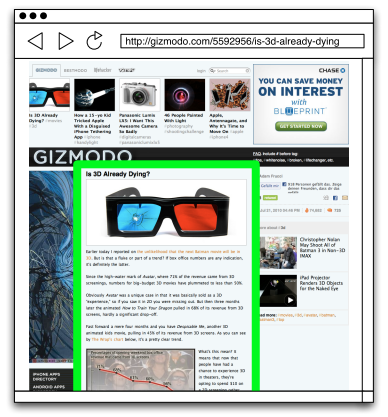
\includegraphics[width=4in]{img/webpagecontentextractor.png}
\caption{Article content of a web page marked with a green box  \cite{katz2010diploma}.}
\label{fig:webpagecontentextractor}
\end{figure}

To perform this kind of extraction we could use wrapper approaches which are explained in more detail in \cite{ckgs2006}. However, these approaches require manual wrapper construction or semi-supervised learning which is too cumbersome.
Another approach would be to detect the template of the web page and get only the contents of the main block (the green box). Template detection usually works by comparing one page with several other pages of the same domain to find the fix and changeable contents. This however requires several http requests and therefore more time and bandwidth.
In Palladian we use an approach that is based on a hierarchical analyzis of the web page's DOM tree. Each DOM element is analyzed and ranked based on the length of the contained text, the link density, and the frequency of other elements in relation to the text length. Longer text fragments usually indicate a relevant part of the article, while a high link density is more likely to indicate that the analyzed element is part of the navigation for example. Also the attributes ``id'' and ``class'' are analyzed. If the attribute values contain keywords such as ``entry'', ``content'', or ``text'', the element is more likely to contain relevant content as if the attribute values contain keywords such as ``header'', ``footer'', or ``sidebar''. The implementation of the web page content extraction adopted great parts of the Firefox extension ``Readability''\footnote{\url{http://lab.arc90.com/experiments/readability/}}. The used heuristics in Readability have shown to be quite accurate for a wide range of web pages. Listing~\ref{listing:usePageContentExtractor} gives a short usage example.

\begin{codelisting}
\begin{lstlisting}[label=listing:usePageContentExtractor,caption=Using the PageContentExtractor.,frame=tb]
PageContentExtractor extractor = new PageContentExtractor();

// this method is heavily overloaded and accepts various types of input
String url = "http://www.wired.com/gadgetlab/2010/05/iphone-4g-ads/";
extractor.setDocument(url);

// get the main content as text representation
String contentText = extractor.getResultText();

// get the main content as DOM representation
Document contentDocument = extractor.getResultDocument();

// get the title
String title = extractor.getResultTitle();
\end{lstlisting}
\end{codelisting}

% TODO code snippet

We evaluated our Readability-inspired approach against Boilerpipe\footnote{\url{http://code.google.com/p/boilerpipe/}}, a Java library which is based on the algorithms described in \cite{BoilerplateDetectionShallowTextFeatures}. For evaluation we used the ``L3S-GN1'' data set which is provided by the authors of Boilerpipe and consists of 621 manually annotated web pages with news articles from 408 different sites. The annotations which were assigned by humans categorize areas of web pages into different groups ``Headline'', ``Full text'',  ``Supplemental'', ``Related content'', ``Comments'' and  ``Not content'', where ``Full text'' represents the main article content of a web page (green box in figure~\ref{fig:webpagecontentextractor}).

We used both content extraction approaches on the data set and scored their results by comparing their extracted text content with the human extracted content using Levenshtein\footnote{\url{http://www.merriampark.com/ld.htm}} similarity. Table~\ref{tab:pageContentExtractionResults} shows the results of our evaluation. The number of wins denotes how many times one approach achieved a better e. g. more similar result than the other.


\begin{table}[ht]
\centering
\begin{tabular}{|l|c|c|c|}
	\hline
	System & Average Similarity & \# Wins & \# Errors \\ 
	\hline
	Boilerpipe (\texttt{ArticleExtractor}, version 1.1) & 88.93\% & 143 & 6 \\ 
	\hline
	Palladian (SVN revision 1444) & 90.91\% & 474 & 2 \\ 
	\hline
\end{tabular}
\caption{Evaluation results for web page content extraction approaches.}
\label{tab:pageContentExtractionResults}
\end{table}

\subsection{Named Entity Recognition}

{\it Named Entity Recognition} (NER) is the task of recognizing and disambiguating known and unknown entities in documents. In order to understand the task we need to understand what an {\it entity} is. An entity is a collection of rigidly designated chunks of text that refer to exactly one or multiple identical, real or abstract concept instances. These instances can have several aliases and one name can refer to different instance \cite{webknoxblogne}. So for example ``Iron Man 2'' and ``Iron-Man 2'' are two different chunks of text which however refer to the same movie. Common types of entities are people (e.g. ``Jim Carrey''), locations (e.g. ``Los Angeles''), and organizations (e.g. ``Google Inc.'').

A named entity recognizer is therefore a system or technique that tries to detect entities in a given natural language text. For example, an NER system that is used to detect people, locations, and organizations should be able to find the bold entities in the following text:

\textbf{Bill Gates} founded \textbf{ Microsoft} with \textbf{ Paul Allen} in 1975 in \textbf{ Albuquerque, New Mexico}. The headquarter is located in \textbf{ Redmond, Washington} and the company is led by CEO \textbf{ Steve Ballmer}.

\subsubsection{Taggers}
Palladian wraps 8 Named Entity Recognizers using a single interface making it easier to test and substitute them in real world applications.

\paragraph{Alchemy} The Alchemy API is a web-based service that also offers Named Entity Recognition. Using this NER requires the application to have a developer key and Internet access. Alchemy covers a wide range of concepts. For more details see \url{http://www.alchemyapi.com/api/entity/types.html} or the JavaDoc.

\paragraph{Illinois Learning-based Java} Students from the University of Illinois developed this Recognizer \cite{illinoisccg}. The recognizer comes with a large set of lists that help the recognizer to tag concepts such as corporations, countries, jobs, movies, people, songs, and more. More information can also be found on \url{http://l2r.cs.uiuc.edu/~cogcomp/asoftware.php?skey=FLBJNE}.

\paragraph{Julie} The Julie Lab of the University of Jena added a named entity recognizer to their NLP toolsuite \cite{hahn2008overview}. The tagger is based on conditional random fields and comes with three models from the biomedical domain. Other models can however trained using Palladian. For more information see the pdf which is contained in their stand-alone download from \url{http://www.julielab.de/Resources/Software/NLP+Tools/Download/Stand_alone+Tools.html}.

\paragraph{LingPipe} The LingPipe library \cite{lingpipe} also offers an NER. Unfortunately the tagger comes with no models. Models for each desired concept need to be trained manually. More information can be found on \url{http://alias-i.com/lingpipe/demos/tutorial/ne/read-me.html}.

\paragraph{OpenCalais} The Open Calais API \cite{opencalais} is a web-based service that also offers Named Entity Recognition. The service requires a developer key and access to the Internet. Open Calais covers many concept as covered on the documentation \url{http://www.opencalais.com/documentation/calais-web-service-api/api-metadata/entity-index-and-definitions} and in the JavaDoc.

\paragraph{OpenNLP} The OpenNLP toolkit \cite{opennlp} provides a maximum entropy based approach for named entity recognition. The toolkit comes with a small set of pre-trained models covering concepts such as locations, organizations, and persons. More details can be found in the JavaDoc.

\paragraph{Stanford} As part of the Stanford NLP library \cite{stanfordnlp} \cite{finkel2005stanfordner} developed a named entity recognizer that is based on conditional random fields (CRF). The tagger was trained on the CoNLL 2003 data and comes with a small set of classifiers that can recognize persons, locations, and organizations. For more details see \url{http://www-nlp.stanford.edu/software/crf-faq.shtml} and the JavaDoc.

\paragraph{TUD} The TUD named entity recognizer was developed at the Dresden University of Technology. The recognizer is based on a list lookup and dictionary classification approach. So far no trained models exist for this tagger.

\subsubsection{Tagging a Text}
To use an NER you need two things: A text that you want to tag and a model for the tagger that has been trained to recognize the entities you want to find in the given text.
The tagging works the same for all NERs and is shown in Listing \ref{listing:useNER}.

\begin{codelisting}
\begin{lstlisting}[label=listing:useNER,caption=Tagging a text using a named entity recognizer.,frame=tb]
// create the tagger
NamedEntityRecognizer ner = new TUDNER();

// the text to be tagged
String inputText = "The iphone 4 is the successor of the iphone 3gs.";

// the path to the model which should be used for tagging
String modelPath = "data/models/tudner/phone.model";

// tag the text using the specified model
String taggedText = ner.tag(inputText, modelPath);
System.out.println(taggedText);
// desired output
// The <PHONE>iphone 4</PHONE> is the successor
// of the <PHONE>iphone 3gs</PHONE>.

// avoid loading the model each time using it
ner.loadModel("data/models/tudner/phone.model");
ner.tag(inputText);
\end{lstlisting}
\end{codelisting}

In order to find out which tags were trained for the model you can create a meta file with one tag name per line, give it the same name as the model adding the suffix ``\_meta'' and save it as a text file next to the model. Listing \ref{listing:nerMeta} shows how you can get a list of tags that a model can apply.

\begin{codelisting}
\label{listing:nerMeta}
\begin{lstlisting}[label=listing:nerMeta,caption=Reading a model's meta data.,frame=tb]
// create the tagger
NamedEntityRecognizer ner = new TUDNER();

// the meta file must be called phone_meta.txt
List<String> tags = ner.getModelTags("data/models/tudner/phone.model");

// print the tags to the console
CollectionHelper.print(tags);
\end{lstlisting}
\end{codelisting}

\subsubsection{Training a Tagger}

Some of the available taggers come with trained models that can be used to detect entities. However, the concepts they were trained for might not be sufficient for the application you have in mind, therefore, you need to create your own training set with entities from your domain and learn a tagger using that data. This section explains which tagging formats are available and how models for the available taggers can be trained.

First we start with the tagging formats which can be used to create a training set.

\paragraph{Tagging Formats}
Many tagging types have been developed which makes interoperability between different systems harder. Palladian can handle many of these formats and is able to transform a tagged text within these formats. 

The different tagging are explained in this section using the same example text: ``Bill Gates founded Microsoft in 1975.''.

\subparagraph{Slash} The slash notation tags a given text with a slash and the tag right after the word. The sample text in the slash notation would look as show below.

\begin{verbatim}
Bill/PERSON Gates/PERSON founded Microsoft/ORG in 1975/DATE.
\end{verbatim}

\subparagraph{Bracket} The bracket notation wraps the word in brackets. The sample tags would look as shown below.

\begin{verbatim}
[Bill Gates PERSON] founded [Microsoft ORG] in [1975 DATE].
\end{verbatim}

\subparagraph{Column (BIO)} The column notation is one of the most widely used. For example the CoNLL NER dataset uses this format. The text is tokenized and on each line of the tagged text there is only one token (word) with its related tag separated by a space or tab. The BIO format means \textbf{ B}eginning, cont\textbf{ I}nue, and \textbf{ O}utside. The BIO format can help to distinguish entities of the same type that are written close together.

The sample text in the column format would look as shown below. The ``O'' tag stands for ``outside'', that is no matching tag has been found.

\begin{verbatim}
Bill PERSON
Gates PERSON
founded O
Microsoft ORG
in O
1975 DATE
. O
\end{verbatim}

The sample text in the column BIO format would look as shown below.

\begin{verbatim}
Bill B-PERSON
Gates I-PERSON
founded O
Microsoft B-ORG
in O
1975 B-DATE
. O
\end{verbatim}

If we had another person name right after the first one, our tagger might think that it was only one person if we use the column notation. In the column BIO notation, both persons could be distinguished because the second one would start with B-PERSON.

\subparagraph{XML} The XML notation is very common too and is the favored one in Palladian. Similarly to the brackets notation, the XML notation wraps the word in an XML tag. The sample tags would look as shown below.

\begin{verbatim}
<PERSON>Bill Gates</PERSON> founded <ORG>Microsoft</ORG> in <DATE>1975</DATE>.
\end{verbatim}

\subparagraph{List} The list notation is a separate file which contains references to the marked entities in the text. For each marked entity it contains its name, its start and stop index, and its tag. The sample list file for the sample text would look as shown below.

\begin{verbatim}
Bill Gates, 0-10, PERSON
Microsoft, 19-28, ORG
1975, 32-36, DATE
\end{verbatim}

The FileFormatParser can transform the formats back and forth as shown in Figure \ref{fig:taggingFormats}. As you can see, we can transform every format to the XML notation which will be used to create an annotation list for the tagged text.

\begin{figure}[ht!]
\centering
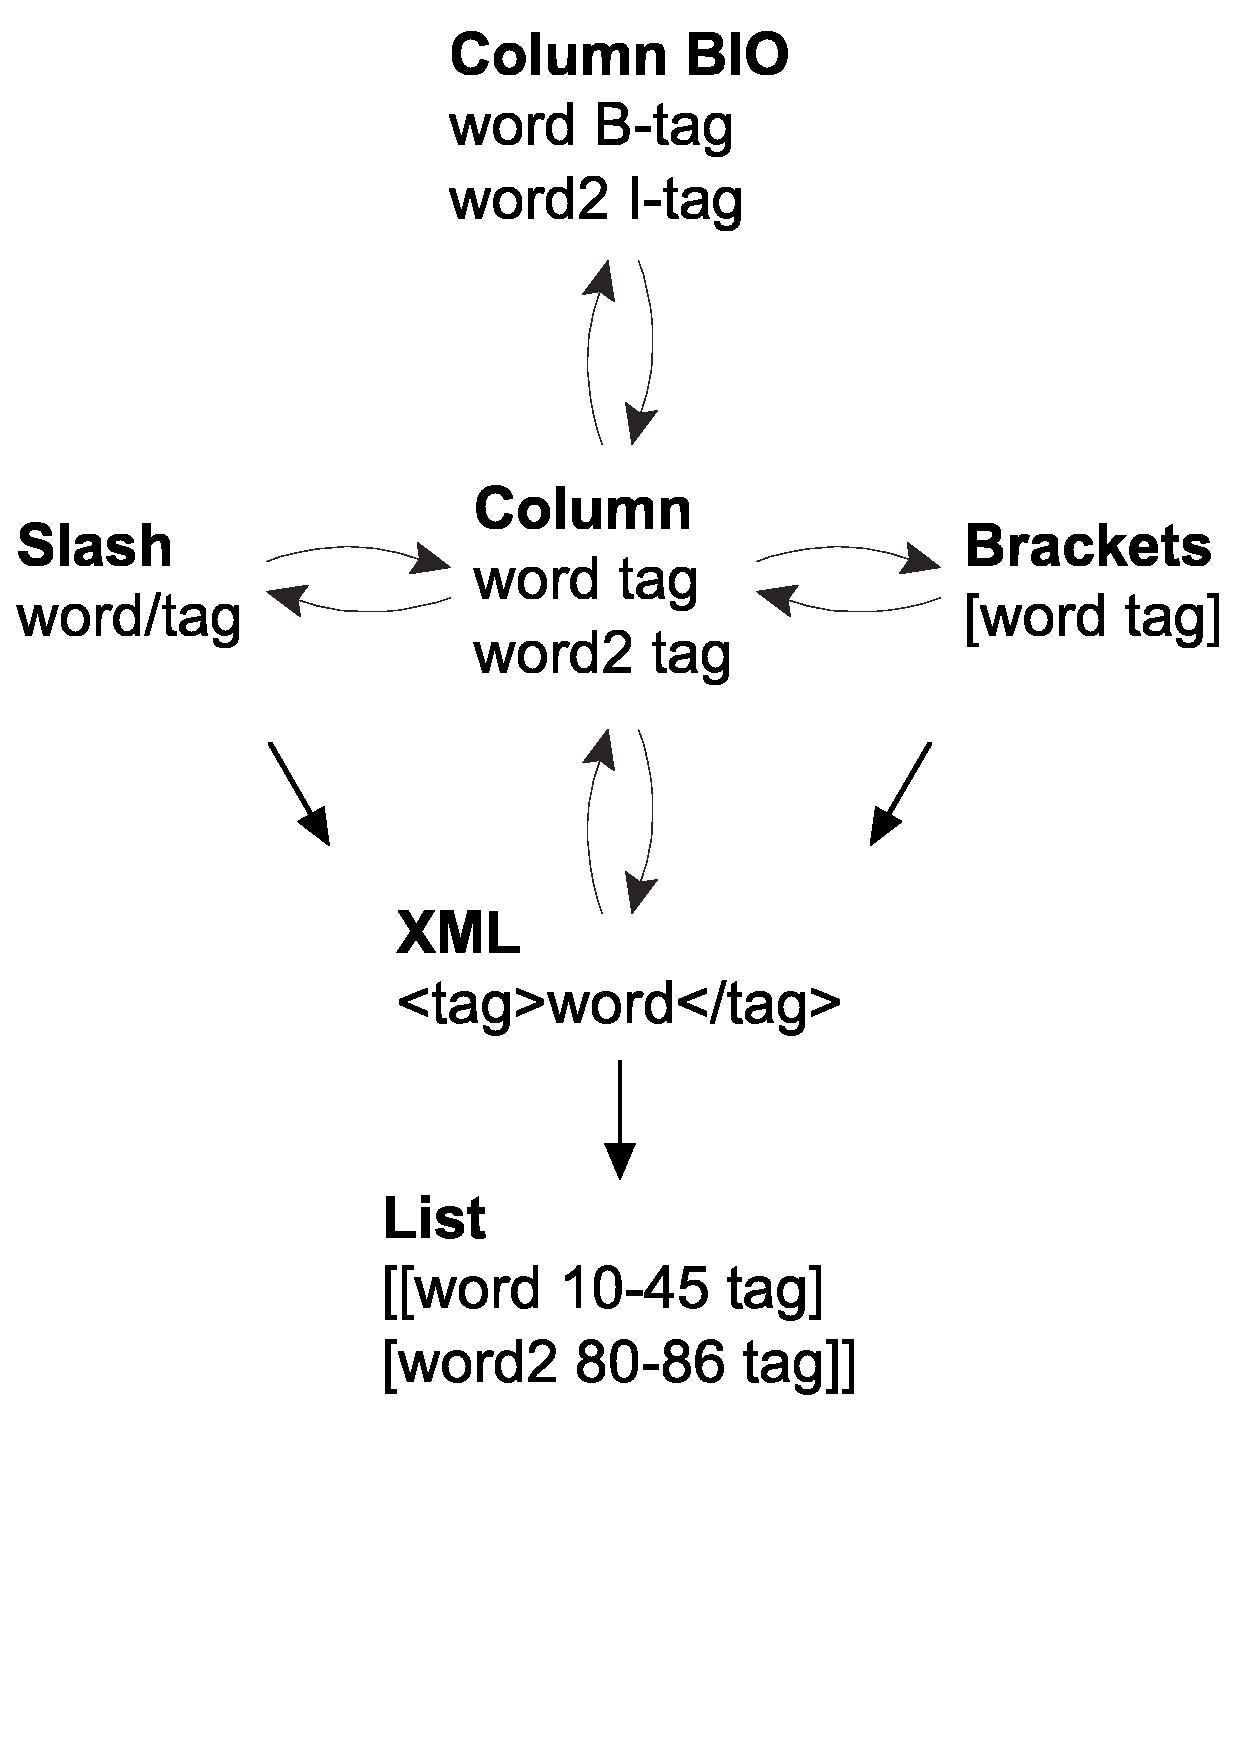
\includegraphics[width=0.5\textwidth]{img/taggingFormats.pdf}
\caption{Possible transformation of tagging formats.}
\label{fig:taggingFormats}
\end{figure}

\paragraph{Using the training set}
Once you have created your training set, you should use the FileFormatParser to transform it into a tab separated column tagging format (if it isn't in this format already).

It is not possible to train a model for the web-based taggers Alchemy and OpenCalais. All other taggers can be trained using the train method, that requires the training file and a model configuration parameter which is different for each tagger.

Let us assume we want to train a model for each trainable tagger to recognize mobile phone names. You should have tagged training data in column separated form as shown below. Usually, the more training data you have, the more stable the trained model. This training data is stored in a tsv file called ``phoneTraining.tsv''.

\begin{verbatim}
The	O
iphone	PHONE
4	PHONE
sells	O
very	O
well O
.	O
\end{verbatim}

Each tagger can be trained as shown in Listing \ref{listing:trainNER}. The only parameter which is used differently for each tagger is the ``modelConfig''. Table \ref{tab:nerConfig} shows what that parameter means for each trainable recognizer.

\begin{table}[ht]
\centering
\begin{tabularx}{\linewidth}{|l|X|X|}
\hline
NER		& Parameter meaning & Example \\
\hline
IllinoisLbjNER	& Path to a configuration file, in this file you can specify which features and parameters should be used and where the trained model should be saved &	.../illinoisner/baselineFeatures.config \\
\hline
JulieNER	& Output path for the trained model. You can add a further parameter with the path to a configuration file, in this file you can specify which features and parameters should be used &	.../juliener/phoneModel.mod and [.../juliener/tutorial/featconfig.conf] \\
\hline
LingPipeNER	& Output path for the trained model &	.../lingpipe/phone.model \\
\hline
OpenNLPNER	& Output path for the trained model, the filename must follow the format ``openNLP\_TAG.bin.gz'' since you can only train one tag per model &	.../opennlp/openNLP\_phone.bin.gz \\
\hline
StanfordNER	& Path to a configuration file, in this file you can specify which features and parameters should be used and where the trained model should be saved &	.../lingpipe/training/austen.prop \\
\hline
TUDNER	& Output path for the trained model &	.../tudner/phoneModel.model \\
\hline
\end{tabularx} 
\caption{Configuration parameters to train named entity recognizers.}
\label{tab:nerConfig}
\end{table}

\begin{codelisting}
\begin{lstlisting}[label=listing:trainNER,caption=Train a named entity recognizer.,frame=tb]
NamedEntityRecognizer ner = new StanfordNER();
boolean successful = ner.train("phoneTraining.tsv", modelConfig);
String output = "successful";
if (!successful) {output = "not successful";}
System.out.println("Training of "+ner.getName()+" was "+output);
\end{lstlisting}
\end{codelisting}

\subsubsection{Evaluating a Tagger}
To see how good a trained tagger performs, we need test data which is tagged in the same manner as the training data. There are different versions of how to evaluate the performance. Let's go through them using an example. For example, let us assume that a human expert created the following markup \cite{nadeau2007yooname}:

\begin{verbatim}
Unlike <PERSON>Robert</PERSON>, <PERSON>John Briggs Jr</PERSON> contacted 
<ORG>Wonderful Stockbrockers Inc</ORG> in <LOCATION>New York</LOCATION> 
and instructed them to sell all his shares in <ORG>Acme</ORG>.
\end{verbatim}

Furthermore, let us assume that a NER system created the following markup \cite{nadeau2007yooname} for the same text:

\begin{verbatim}
<LOCATION>Unlike</LOCATION> Robert, <ORG>John Briggs Jr</ORG> contacted 
Wonderful <ORG>Stockbrockers</ORG> Inc <DATE>in New York</DATE> and 
instructed them to sell all his shares in <ORG>Acme</ORG>.
\end{verbatim}

The only correct match between the correct solution and the NER system output is \verb$<ORG>Acme</ORG>$, all other markups are some kind of errors.

\paragraph{Error Types}
In classification tasks it is often possible to determine the true positives, false positives etc. but in NER it can sometimes help to be more precise about the classes. For example, two false positives are not necessarily equally wrong. Consider a system that had to tag person names in text, and it tagged ``A good start'' and ``Jim Carrey was'' as persons. While the first occurrence is obviously totally wrong, the second has to be considered wrong too but the system only did not find the right hand boundary correctly and tagged the word ``was'' too.
In the previous example we can see five different errors an NER system can make \cite{manning2006nererrors}. The errors are shown and explained in the Table \ref{tab:nererrors} \cite{nadeau2007yooname}.

\begin{table}[ht!]
\centering
\begin{tabularx}{\linewidth}{|X|X|X|}
\hline
Correct Solution	 		& 	System Output	& Error\\
\hline
\hline
Unlike						&	\verb$<LOCATION>Unlike</LOCATION>$	&	The system tagged an entity where there is none.\\
\hline
\verb$<PERSON>Robert</PERSON>$	&	Robert								& 	The system missed to tag an entity.\\
\hline
\verb$<PERSON>John Briggs Jr$ \verb$</PERSON>$	& \verb$<ORG>John Briggs Jr</ORG>$	&	The system tagged the entity but classified it incorrectly.\\
\hline
\verb$<ORG>Wonderful$ \verb$Stockbrockers Inc</ORG>$	&	\verb$<ORG>Stockbrockers</ORG>$	&	The system tagged the entity but the boundaries are wrong.\\
\hline
\verb$<LOCATION>New York$ \verb$</LOCATION>$	&	\verb$<DATE>in New York</DATE>$	&	The system found an entity but classified it incorrectly and got the boundaries wrong.\\
\hline
\end{tabularx} 
\caption{NER features \cite{nadeau2007yooname}.}
\label{tab:nererrors}
\end{table}

Due to the variety of combinations to use the error types, three main evaluation methods have evolved during the years.

\paragraph{Exact-Match Evaluation}
The exact-match evaluation is the most simple one and does not take the different error types into account. A correct assignment must have the boundaries and the classification correct. The final score for the NER system is a micro-averaged f-measure (MAF). The NER system from the example would get the following scores.
\begin{itemize}
\item Precision = Correct / Total Assigned = 1 / 5 = 20\%
\item Recall = Correct / Total Possible = 1 / 5 = 20\%
\item MAF = 20\%
\end{itemize}

\paragraph{MUC Evaluation}
The MUC evaluation method takes all five errors from Table \ref{tab:nererrors} into account and scores a system along two axis, the TYPE and the TEXT axis. If an entity was classified correctly (regardless of the boundaries) the TYPE is assigned correct. If an entity was found with the correct boundaries (regardless of its type) the TEXT is assigned correct. For both axis, three measures are kept: the number of possible entities (POS), the number of actual assigned entities by the system (ACT) and the number of correct answers by the system (COR).
MUC als uses the MAF as the final score for the NER system. As the usual f-measure, also the micro-averaged f-measure is the harmonic mean between precision and recall.
For the example we can calculate the MUC score for the system as follows.
\begin{itemize}
\item COR = 4 (2 times TYPE correct, 2 times TEXT correct)
\item ACT = 10 (5 times TYPE assigned, 5 times TEXT assigned)
\item POS = 10 (5 times TYPE, 5 times TEXT)
\item Precision = COR / ACT = 4 / 10 = 40\%
\item Recall = COR / POS = 4 / 10 = 40\%
\item MAF = 40\%
\end{itemize}

Listing \ref{listing:evaluateNER} shows how we can programmatically evaluate a tagger. 

\begin{codelisting}
\begin{lstlisting}[label=listing:evaluateNER,caption=Evaluating the performance of a named entity tagger.,frame=tb]
// initialize the tagger
NamedEntityRecognizer ner = new TUDNER();

// the path to the test data
String testFilePath = "testData.xml";

// the path to the model that we want to evaluate
String modelPath = "data/models/tudner/phone.model";

// store the evaluation results in an object
EvaluationResult eResult = null;

// evaluate the model using the test data
eResult = ner.evaluate(testFilePath, modelPath, TaggingFormat.XML);

// print out the evaluation result
System.out.println(eResult);

// get interesting values in exact match and MUC mode
String r1 = "F1 Exact: " + eResult.getF1(EvaluationResult.EXACT_MATCH);
String r2 = "F1 MUC: " + eResult.getF1(EvaluationResult.MUC);
System.out.println(r1);
System.out.println(r2);
\end{lstlisting}
\end{codelisting}

\subsection{Web Page Age Detection}
The age of a web page can often be a useful indicator about the freshness of the information. It might also be used in classification or ranking of web documents. Palladian is able to detect the age of many web pages by using four main techniques:
\begin{enumerate}
\item Reading the \textbf{ HTTP header} of a web page and look for the date that the page has changed. Although this information is often absent of incorrect it sometimes is the only date we get.
\item Recognize a date in the \textbf{ URL} of the web page. Especially blogs use the URL style which often reads similar to ``http://domain.tld/posts/YYYY/MM/PostName''. In these cases the date in the domain is a very good indicator of the web page's age.
\item Recognizing and ranking dates in the \textbf{ structure and content} of the web page. Especially news pages start or end their news posts with the location and the date that the event they are reporting about happened. Since many dates might be found in the content it is necessary to rank them among each other. This is done using indicators such as the nearness to certain keywords such as ``published'' for example.
\item Searching for \textbf{ inbound links from archives}. Some web pages can be found in archives with a date. If none of the other techniques returns valuable results it is possible to look up the URL in an archive, although the chances to find it are quite low.
\end{enumerate}

Listing \ref{listing:dateRecognizer} shows how to detect the age of a web page. For more information on the algorithms used, see \cite{gregor2010bachelor}. You can also check out the functionality of the web page age detection online at \url{http://www.webknox.com/wi#detectAge}.

% TODO out of sync with code!
\begin{codelisting}
\begin{lstlisting}[label=listing:dateRecognizer,caption=Detecting the age of a web page.,frame=tb]
// the URL of the page we want to know the age from
String url = "http://www.bbc.co.uk/news/world-europe-11432849";

// ExternalSearch is a boolean to switch on and off reference and
// archive techniques. Standard should be false (off).
boolean externalSearch = false;

// get the highest ranked date for this web page
ExtractedDate date = WebPageDateEvaluator
				.getBestRatedDate(url, externalSearch);

// print the extracted date (should be 29.09.2010)
System.out.println(date);
\end{lstlisting}
\end{codelisting}

\subsection{FAQ Extractor}
\textit{ FAQs} are frequently asked questions that are often found on web pages in a structured form. Basically there are three types how the FAQ can be structured:
\begin{enumerate}
\item \textbf{ Internal Link} In the beginning of the page, there is a list of questions that each link to the corresponding answer in on the same page.
\item \textbf{ External Link} In the beginning of the page, there is a list of questions that each link to the the web page that contains the answer.
\item \textbf{ No Link} Each question is immediately followed by its answer.
\end{enumerate}

Palladian can handle many FAQs that follow the first or third structure. First, the algorithm detects the XPaths to the questions and then it tries to extract all content between the current and the next question as the answer for the current question.

Listing \ref{listing:faqExtractor} shows how the FAQExtractor can be used programatically. You can also check out the functionality of the FAQ Extractor online at \url{http://www.webknox.com/wi#extractFAQ}.

\begin{codelisting}
\begin{lstlisting}[label=listing:faqExtractor,caption=Extract an FAQ from a web page.,frame=tb]
// create a list of question answer pairs
ArrayList<QA> qas = null;

// the URL that contains the FAQ
String url = "http://blog.pandora.com/faq/";

// start extracting question and answers from the URL
qas = QAExtractor.getInstance().extractFAQ(url);

// print the extracted questions and answers
CollectionHelper.print(qas);
\end{lstlisting}
\end{codelisting}

\subsection{Fact Extraction}
The FactExtractor can be used to detect facts in tables on web pages given a URL and optionally a small set of seed attribute names that help the extractor. The FactExtractor constructs all XPaths to the seed attributes and compares them. If it recognizes a similarity it concludes that the XPaths that are similar for the seed attributes might also point to other attributes on the page. In case of attributes that are listed in simple tables this approach works pretty well, if the attributes are presented in a more complicated way, the fact extractor might not find anything.

You can also check out the functionality of the FactExtractor online at \url{http://www.webknox.com/wi#extractFacts}.

\begin{codelisting}
\begin{lstlisting}[label=listing:factExtraction,caption=Extract a list of facts from a web page.,frame=tb]
// the URL of the facts
String url = "http://en.wikipedia.org/wiki/Nokia_N95";

// the concept of the attributes
Concept concept = new Concept("Mobile Phone");

// a small list of seed attributes
Set<Attribute> seeds = new HashSet<Attribute>();
int attributeType = Attribute.VALUE_STRING;
seeds.add(new Attribute("Second camera", attributeType, concept));
seeds.add(new Attribute("Memory card", attributeType, concept));
seeds.add(new Attribute("Form factor", attributeType, concept));

// detect the facts using the seeds from the URL
ArrayList<Fact> detectedFacts = null;
detectedFacts = FactExtractor.extractFacts(url, seeds);
		
// print the extracted facts
CollectionHelper.print(detectedFacts);
\end{lstlisting}
\end{codelisting}

\section{Retrieval}

\subsection{Source Retriever}
The source retriever is a module that can query a number of sources such as search engines and web pages with terms and retrieve matching results.
\subsubsection{Basic Features}
Basic features are:
\begin{itemize}
\item Query the Google search engine (unlimited queries, top 64 results only).
\item Query Yahoo search engine (5000 queries per IP and day, top 1000 results).
\item Query Bing search engine (unlimited)
\item Query Hakia search engine.
\item Query Twitter.
\item Query Google Blog search.
\item Query Textrunner web page.
\end{itemize}
Some of the search APIs require API keys which must be specified in the config/apikeys.conf file. See \ref{sec:apikeys.conf} for more information.

\subsubsection{How To}
\label{sec:howto}
The following code snippet shows how to initialize the source retriever and get a list of (English) URLs from the Bing search engine for the exact search ``Jim Carrey''.
\begin{codelisting}
\begin{lstlisting}[caption=Retrieving result URLs from a search engine.,frame=tb]
// create source retriever object
SourceRetriever s = new SourceRetriever();
		
// set maximum number of expected results 
s.setResultCount(10);
		
// set search result language to english
s.setLanguage(SourceRetrieve.LANGUAGE_ENGLISH);
		
// set the query source to the Bing search engine 
s.setSource(SourceRetrieverManager.BING);
		
// search for "Jim Carrey" in exact match mode (second parameter = true)
List<String> resultURLs = s.getURLs("Jim Carrey", true);
		
// print the results
CollectionHelper.print(resultURLs);	
\end{lstlisting}
\end{codelisting}

%\subsection{RankAggregation}

\subsection{Web Crawler}
The web crawler can be used to crawl domains or just retrieve the cleansed HTML document of a single web page.

\subsubsection{Basic Features}
Basic functionalities include:
\begin{itemize}
\item Download and save contents of a web page.
\item Automatically crawl in- and/or outbound links from web pages.
\item Use URL rules for the crawling process.
\item Extract title, description, keywords and body content of a web page.
\item Remove HTML, SCRIPT and CSS tags.
\item Find a sibling page of a given URL.
\item Switch proxies after a certain number of requests to avoid being blocked.
\end{itemize}

\subsubsection{How To}
The following code shows how to instantiate a simple crawler that starts at http://www.dmoz.org and follows all in- and outbound links. The URL of each crawled page is printed to the screen. The crawler will use 10 threads, changes the proxy after every third request and stops after having crawled 1000 pages. Instead of setting the parameters using the code, we can also specify them in the config/crawler.conf file. See \ref{sec:classification.conf} for more information.

\begin{codelisting}
\begin{lstlisting}[caption=Using the web crawler.,frame=tb]
// create the crawler object
Crawler crawler = new Crawler();

// create a callback that is triggered for every crawled page
CrawlerCallback crawlerCallback = new CrawlerCallback() {
	@Override
	public void crawlerCallback(Document document) {
		// TODO do something with the page
		System.out.println(document.getDocumentURI());
	}
};
crawler.addCrawlerCallback(crawlerCallback);

// stop after 1000 pages have been crawled (default is unlimited)
crawler.setStopCount(1000);

// set the maximum number of threads to 10
crawler.setMaxThreads(10);

// the crawler should automatically use different proxies
// after every 3rd request (default is no proxy switching)
crawler.setSwitchProxyRequests(3);

// set a list of proxies to choose from
List<String> proxyList = new ArrayList<String>();
proxyList.add("83.244.106.73:8080");
proxyList.add("83.244.106.73:80");
proxyList.add("67.159.31.22:8080");
crawler.setProxyList(proxyList);

// start the crawling process from a certain page,
// true = follow links within the start domain
// true = follow outgoing links
crawler.startCrawl("http://www.dmoz.org/", true, true);
\end{lstlisting}
\end{codelisting}

\subsection{Web Feeds}
Palladian's \texttt{ws.palladian.web.feeds} package offers various functionalities for tasks related to RSS and Atom web feeds. The most important classes include:

\begin{itemize}

	\item \texttt{FeedDownloader} can be used for retrieving web feeds. The class basically wraps ROME library~\cite{rome} for feed parsing but adds some additional techniques and fallbacks for parsing non-standard and malformed feeds, which ROME normally cannot parse.

	\item \texttt{FeedReader} is responsible for continuously aggregating web feeds using various different algorithms to predict feed's update behaviours.

	\item \texttt{FeedDiscovery} allows searching for web feeds using standard web search engines like Yahoo! and the so called ``autodiscovery'' feature\footnote{\url{http://diveintomark.org/archives/2003/12/19/atom-autodiscovery} (also works for RSS)}, to detect feeds on web pages.

	\item \texttt{FeedDatabase} implements the feed's package persistence layer using a relational database. The necessary MySQL database schema can be found in \texttt{config/feedsDbSchema.sql}\footnote{You can use phphMyAdmin or MySQL command line utilities to import the schema into your database.}.

	\item \texttt{FeedImporter} is used for adding new web feeds to the database.

	\item The class \texttt{Feed} and its associated \texttt{FeedItem}s model a web feed's data structure.

\end{itemize}

Code Listing~\ref{listing:feeds} gives a minimal sample use case employing the described classes.

\begin{codelisting}
\begin{lstlisting}[caption=Using the \texttt{feeds} package.,frame=tb,label=listing:feeds]
// search feeds for "Porsche 911"
FeedDiscovery feedDiscovery = new FeedDiscovery();
feedDiscovery.setSearchEngine(SourceRetrieverManager.YAHOO_BOSS);
feedDiscovery.addQuery("Porsche 911");
feedDiscovery.setResultLimit(100);
feedDiscovery.findFeeds();
Collection<String> feedUrls = feedDiscovery.getFeeds();
CollectionHelper.print(feedUrls);

// download a feed
FeedDownloader feedDownloader = new FeedDownloader();
Feed feed = feedDownloader.getFeed("http://rss.cnn.com/rss/edition.rss");
List<FeedItem> feedItems = feed.getItems();
CollectionHelper.print(feedItems);

// initialize the FeedDatabase for storing the data
FeedStore feedStore = new FeedDatabase();

// add some feed URLs to the database
FeedImporter feedImporter = new FeedImporter(feedStore);
feedImporter.addFeeds(feedUrls);

// start aggregating news for the feeds in the database
// (this is an infinite loop)
FeedReader feedReader = new FeedReader(feedStore);
feedReader.aggregate(false);
\end{lstlisting}
\end{codelisting}


\section{Preprocessing}
\subsection{Tokenization}
A \textit{Token} is a sequence of characters that can be categorized according to the tokenization rules. \textit{Tokenization} is the process of transforming a text into a sequence of tokens. Table \ref{tab:tokenTypes} shows example token types. The text ``Today I lost \$1000 dollar playing poker.'' could consists of 8 tokens for example. What token types exist depend on the application. The dollar sign could be a single token for example. Palladian uses regular expressions to perform the tokenization.

\begin{table}[ht!]
\centering
\begin{tabular}{|l|l|}
\hline
Character sequence		& Token type \\
\hline
many			& word \\
\hline
\$1000		& amount of money  \\
\hline
26.09.2010	& date \\
\hline
.				& punctuation \\
\hline
\end{tabular} 
\caption{Example types of tokens.}
\label{tab:tokenTypes}
\end{table}

One can also see each sentence of a text as a token, in this case the tokenization process is called sentence splitting as explained int he next section.

\subsection{Sentence Splitting}
Palladian has a rudimentary implementation for the common need for sentence splitting. Palladian implementation works with hand-crafted rules and thus does not require a model. Sentences try to be splitted on periods, question marks, and exclamation marks but there are also rules that try to prevent splitting sentences at ellipses. For example, the following is online one sentence although it contains several periods: ``Sometimes sentenes contain many periods...really!''.

The following code shows how the sentence splitting can be used:
\begin{codelisting}
\begin{lstlisting}[caption=Using the sentence splitter.,frame=tb]
String inputText = "This is a sentence. This is another one!";
List<String> sentences = Tokenizer.getSentences(inputText);
CollectionHelper.print(sentences);
// prints:
// This is a sentence
// This is another one!
\end{lstlisting}
\end{codelisting}

You can also get a specific sentence by providing a phrase that is part of the sentence using the $getSentence$ method.

\subsection{Creating N-Grams}
\label{sec:ngrams}

N-grams are sets of tokens of the length n. We can distinguish two main types of n-grams:

\begin{enumerate}
\item \textbf{Character level n-grams} use each character of the string as a token. For example, from the string ``It is sunny'' we can create the following set of 3-grams: ${it ,t i, is,is ,s s, su,sun,unn,nny}$. The number of n-grams in a set can be calculated as $ngrams = numberOfTokens - n + 1$. In our example that means $9 = 11 - 3 + 1$.
\item \textbf{Word level n-grams} use each word (separated with white space) of the string as a token. For example, from the string ``It is so nice and sunny today'' we can create the following set of 3-grams: ${It is so,is so nice,so nice and,nice and sunny,and sunny today}$. The number of n-grams in a set can be calculated as $ngrams = numberOfTokens - n + 1$. In our example that means $5 = 7 - 3 + 1$. If you want to have single words as features for the text classifier you can simply use unigrams or bigrams which are n-grams with $n=1$ or $n=2$ respectively.
\end{enumerate}

The document preprocessor allows you to create a set of n-grams with different length too. For example, you can create all 2-grams, 3-grams, and 4-grams for the given input text.

Listing \ref{listing:ngrams} shows how you can create n-grams from a given text.

\begin{codelisting}
\label{listing:ngrams}
\begin{lstlisting}[label=listing:ngrams,caption=Creating n-grams.,frame=tb]
// the input text that we want to separate into n-grams
String inputText = "a cat runs funnily";

// store a set of n-grams
Set<String> ngrams = null;

// calculate all character n-grams of length 3
ngrams = Tokenizer.calculateCharNGrams(inputText,3);

// calculate all word n-grams of length 3
ngrams = Tokenizer.calculateWordNGrams(inputText,3);

// calculate all character level n-grams of length 3 to 5
ngrams = Tokenizer.calculateAllCharNGrams(inputText,3,5);

// calculate all character word n-grams of length 1 to 3
ngrams = Tokenizer.calculateAllWordNGrams(inputText,1,3);
\end{lstlisting}
\end{codelisting}

\subsection{Noun Pluralization and Singularization}
Palladian is able to transform most English singular nouns to their plural and back. For example, ``city'' becomes ``cities'' and ``index'' becomes ``indices''.

Listing \ref{listing:singularPlural} shows the simple usage of the singularization and pluralization using the WordTransformer class.

\begin{codelisting}
\label{listing:singularPlural}
\begin{lstlisting}[label=listing:singularPlural,caption=Transforming words from singular to plural and vice versa.,frame=tb]
String singular = "city";
String plural = "";
plural = WordTransformer.wordToPlural(singular);
singular = WordTransformer.wordToSingular(plural);
System.out.println(singular);
System.out.println(plural);
// prints:
// cities
// city
\end{lstlisting}
\end{codelisting}

\section{Miscellaneous}
The toolkit contains many helper functionalities for reoccurring tasks in the \texttt{ws.palladian.helper} package. The following code snippet shows several sample usages of some of the functions.

\begin{codelisting}
\begin{lstlisting}[caption=Miscellaneous functions.,frame=tb]
// sort a map by its value in ascending order (2nd parameter = true)
Map m = CollectionHelper.sortByValue(map, true);

// reverse a list
List l = CollectionHelper.reverse(list);

// print the contents of a collection
CollectionHelper.print(collection);

// get the runtime of an algorithm and print it (2nd parameter = true)
long startTime = System.currentTimeMillis();
for (int i = 0; i < 10000; i++) {
	int c = i * 2;
}
DateHelper.getRuntime(t1, true);

// (de) serialization of objects
FileHelper.serialize(obj, "obj.ser");
Object obj = FileHelper.deserialize("obj.ser");

// rename, copy, move and delete files
FileHelper.rename(new File("a.txt"), "b.txt");
FileHelper.copyFile("src.txt", "dest.txt");
FileHelper.move(new File("src.txt"), "dest.txt");
FileHelper.delete("src.txt");

// get files from a folder
File[] files = FileHelper.getFiles("folder");

// zip and unzip a text
FileHelper.zip("text", "zipFile.zip");
String t = FileHelper.unzipFileToString("zipFile.zip");

// perform some action on every line of an ASCII file
final Object[] obj = new Object[1];
obj[0] = 1;

LineAction la = new LineAction(obj) {
  
    @Override
    public void performAction(String line, int lineNumber) {
        System.out.println(lineNumber + ": " + line + " " + obj[0]); 
    }
}
FileHelper.performActionOnEveryLine(filePath, la);

// round a number with a number of digits
double r = MathHelper.round(2.3333, 2);

// remove HTML tags
String r = HTMLHelper.removeHTMLTags("<a>abc</a>",
                                       true, true
                                       true, true);

// trim a string
String t = StringHelper.trim(" _to trim++++");

// reverse a string
String r = StringHelper.reverse("abc");

// encode and decode base64
String e = StringHelper.encodeBase64("abc");
String d = StringHelper.decodeBase64(e);

\end{lstlisting}
\end{codelisting}

\chapter{Where to Go from Here?}
Why go, just stay here :) No, seriously, if you can't find something that you need, there is a list of similar projects in Section \ref{sec:alternativesToPalladian} that you can scan through. If you still can't find it, research the topic, implement the code and commit it back to Palladian.

\section{Referenced Libraries}
Palladian makes excessive use of third party libraries. We do not intend to re-implement code but rather to built on it and create something superior. Here an incomplete list of libraries the toolkit uses:
\begin{itemize}
\item Apache Commons \cite{apachecommons} for many standard tasks in string and number manipulation and more.
\item Fathom \cite{fathom} to measure readability of English text.
\item iText \cite{itext} for creating PDF documents.
\item Jena \cite{jena} for reading and writing ontology files.
\item jYaml \cite{jyaml} to read and write YAML files.
\item Log4j \cite{log4j} for logging.
\item Lucene \cite{lucene} for indexing and making learned models persistent.
\item NekoHTML \cite{nekohtml} to clean up the HTML of web pages in order to process them correctly.
\item ROME \cite{rome} for parsing RSS and Atom feeds.
\item SimMetrics \cite{simmetrics} to calculate similarities of strings.
\item Twitter4j \cite{twitter4j} to query the Twitter API.
\item Weka \cite{hall2009weka} for machine learning.
\end{itemize}

\section{History}
The foundation of Palladian's code came out of the WebKnox project\cite{webknox} that was started in 2008.% Now, components of the Aletheia project\footnote{\url{http://www.aletheia-projekt.de}} and the Effingo project\footnote{\url{http://www.effingo.de}}

The code is in development by students of the Dresden University of Technology. Contributors are:
\begin{itemize}
\item Christopher Friedrich
\item Martin Gregor
\item Philipp Katz
\item Klemens Muthmann
\item Silvio Rabe
\item Sandro Reichert
\item David Urbansky
\item Robert Willner
\item Martin Werner
\item Martin Wunderwald
\item Stephan Zepezauer
\end{itemize}

%\chapter{References}
\bibliographystyle{abbrv}
\bibliography{references}

\end{document}
